\chapter{Vývojářská dokumentace}

\section{Technologie}

Celý systém je naprogramován v rozšířeném objektově orientovaném jazyce {\em Java} (verze~1.6) a drobné části (např. databázové pohledy) ve skriptovacím jazyce {\em JavaScript}. Systém používá dokumentově orientovanou databázi {\em CouchDB}, přístupnou přes rozhraní HTTP (REST API). Spolupráce s databází je zajištěna open-source knihovnou {\em jcouchdb}. Webová aplikace je postavena na frameworku {\em Apache~Wicket}. Produkční verze webové aplikace běží v kontejneru {\em Tomcat}. Pro fulltextové vyhledávání je použit servlet {\em CouchDB~Lucene}, který v sobě integruje vyhledávací engine {\em Lucene} a stará se o jeho napojení na databázi CouchDB. Pro čtení obrázků typu TIFF používáme knihovnu {\em Apache~Sanselan}, o kompilaci a sestavení se stará {\em Apache~Maven}. Zdrojový kód byl vyvíjen v prostředí {\em Eclipse}, nastavení automatického formátování je přiloženo v souboru {\em eclipse\_formatter.xml}.

Zde jsou domovské odkazy na každý zmíněný produkt (platné k datu 1.~dubna~2012):

\begin{itemize}
\item{\bf http://download.oracle.com/javase/}
\item{\bf http://www.tvorba-webu.cz/javascript/}
\item{\bf http://code.google.com/p/jcouchdb/}
\item{\bf https://github.com/rnewson/couchdb-lucene}
\item{\bf http://commons.apache.org/sanselan/}
\item{\bf http://couchdb.apache.org/}
\item{\bf http://wicket.apache.org/}
\item{\bf http://maven.apache.org/}
\item{\bf http://www.eclipse.org/}
\end{itemize}

Během programování bylo dbáno na to, aby byl zdrojový kód přehledný, čitelný, pochopitelný a dobře okomentovaný. Proto v tomto dokumentu nebudeme zacházet do velkých implementačních detailů, protože ty by měly být zřejmé při studiu konkrétní části zdrojového kódu. Implementace zde bude popsána na úrovni konceptů a jednotlivých tříd.

{\bf Poznámka}: Podrobnější dokumentaci k jednotlivým třídám, metodám a proměnným je možné najít v samostatném dokumentu, který je generován přímo z komentářů ve zdrojovém kódu (JavaDoc) a je přiložen jako součást dokumentace.

\subsection{Formát JSON}

Klíčovým formátem dat používaným na různých místech systému Retrobi je strukturovaný textový formát JSON (Javascript object notation). Jak již název napovídá, jedná se o velmi omezenou podmnožinu jazyka Javascript určenou k zápisu strukturovaných dat.

Jazyk JSON je velmi jednoduchý, jeho syntaxe je postavena na dvou základních strukturách: {\em množina párů klíč--hodnota} a {\em seznamu hodnot}. Zde je vypsána jeho gramatika:

\begin{itemize}
\item{objekt ::= \{\} $|$ \{ páry \}}
\item{páry ::= pár $|$ pár , páry}
\item{pár ::= řetězec : hodnota}
\item{pole ::= [$\;$] $|$ [ prvky ]}
\item{prvky ::= hodnota $|$ hodnota , prvky}
\item{hodnota ::= řetězec $|$ číslo $|$ objekt $|$ pole $|$ true $|$ false $|$ null}
\end{itemize}

A zde je příklad krátkého dokumentu:

\begin{verbatim}
{
  "jmeno" : "Karel Čapek",
  "narozen" : {"den" : 9, "mesic" : 1, "rok" : 1890},
  "zamestnani" : ["spisovatel", "novinář", "dramatik"]
}
\end{verbatim}

\subsection{CouchDB}

CouchDB je dokumentově orientovaná databáze přístupná přes HTTP REST API implementovaná ve funkcionalním programovacím jazyce Erlang.

Narozdíl od relačních databází nejsou v CouchDB žádné relace, tabulky, transakce, integritní omezení, ani datové definice. Relace mezi záznamy jsou v aplikaci Retrobi zajištěny až na úrovni aplikace -- vazební proměnné jsou tedy řetězce typu {\bf String} (případně {\bf Set$<$String$>$}) a je v nich uložen klíč vázaného dokumentu (řetězec obsahující {\bf \_id} nebo prázdná hodnota {\bf null}). 

Integrita dat tedy není nijak kontrolována na úrovni databáze. To klade vyšší nároky na kvalitu klientské aplikace, která ale není omezena v tom, co může do databáze uložit. Vedle sebe tak mohou ležet komentáře k lístkům, lístky, uživatelé, schránky a další typy dokumentů. Systém Retrobi nemá datový model tak košatý, aby to nějak zásadně vadilo a převažují výhody zvoleného řešení, kterými jsou jednoduchost, rychlost a schopnost skladovat strukturovaná data s přiloženými obrázky, což přesně lístková kartotéka v současném stavu je.

Dokumenty jsou v databázi CouchDB logicky (nikoliv fyzicky) uloženy ve formátu JSON (Javascript Object Notation), který byl popsán výše. Adresní prostor databáze je plochý, každý záznam má právě jeden unikátní klíč -- řetězec 32 alfanumerických znaků. Dokument v databázi CouchDB má tři speciální proměnné (poznají se tak, že začínají podtržítkem):

\begin{description}
\item[\_id:]{povinné; primární klíč dokumentu (automaticky generovaný nebo ručně zadaný);}
\item[\_rev:]{povinné; revize (slouží pro kontrolu verzí a prevenci update konfliktů);}
\item[\_attachments:]{nepovinné; každý dokument u sebe může mít přiložen libovolný počet pojmenovaných souborů ve formě přílohy (například u lístků jejich naskenované obrázky); tyto přílohy se nenačítají přímo s dokumentem, ale na vyžádání (kvůli jejich velikosti).}
\end{description}

Dokument je z databáze možné načíst buď dle primárního klíče (tedy řetězce {\bf \_id}), nebo využít tzv. {\em pohledy}. Pohledy nad databází CouchDB jsou postaveny na principu {\em map--reduce} a každý pohled je zároveň indexem. Každý databázový pohled se skládá ze dvou funkcí: funkce {\em map} a funkce {\em reduce}, které jsou definovány v jazyce JavaScript.

\begin{itemize}
\item{{\bf Mapovací funkce ({\em map})} je spuštěna pro každý jeden dokument a vyhodnocena; v jejím těle lze zavolat speciální funkci {\bf emit(klíč,~hodnota)}, kterou lze na základě dokumentu vytvořit libovolný počet párů {\em klíč--hodnota}.}
\item{{\bf Redukční funkce ({\em reduce})} je nepovinná funkce, která je spuštěna (pokud je přítomna) pro každý unikátní klíč a množinu hodnot k tomuto klíči přiřazenou; jako vstup přijímá dvojice {\em klíč--hodnota} vytvořené v mapovací funkci {\em map} a jako výstup vrací jednu hodnotu (skalár/objekt/pole), která je poté ke klíči přiřazena místo všech hodnot původních.}
\end{itemize}

Pohledy jsou uloženy v tzv. {\em design dokumentech}, což jsou speciální systémové dokumenty, jejichž klíč začíná řetězcem {\bf \_design/} a respektují strukturu, ve které je dotazovací podsystém CouchDB schopen definice pohledů najít. Vstupním bodem do této definice je hodnota atributu {\bf views}, kde jsou v další podstruktuře uvedeny definice jednotlivých pohledů (těla jejich funkcí {\em map} a {\em reduce}). Tato podstruktura vypadá zhruba takto:

\begin{verbatim}
"views": {
  "VIEW NAME 1": {
    "map": "MAP FUNCTION",
    "reduce": "REDUCE FUNCTION"
  }
}
\end{verbatim}

Dotaz na databázi je v podstatě jen otevření platné URL adresy (požadavek typu GET), která obsahuje tyto údaje:

\begin{itemize}
\item{název {\em design dokumentu} - klíč dokumentu obsahujícího definici požadovaného pohledu;}
\item{název pohledu;}
\item{klíč (nepovinné), který omezí výsledky na zadaný klíč;}
\item{počáteční klíč (nepovinné), který omezí výsledky na ty, jejichž klíče jsou \uv{větší nebo rovny} zadanému počátečnímu klíči (princip řazení je definován v dokumentaci CouchDB);}
\item{konečný klíč (nepovinné), který omezí výsledky na ty, jejichž klíče jsou \uv{menší} než zadaný konečný klíč (lze kombinovat s počátečním klíčem);}
\item{maximální počet výsledků;}
\item{počet výsledků, které se mají od začátku přeskočit.}
\end{itemize}

Po otevření této adresy se CouchDB nejprve podívá, zda je požadovaný pohled aktuální (tedy jsou v něm obsaženy všechny změny dokumentů od jeho poslední aktualizace a nezměnila se jeho definice). 

Pokud pohled aktuální není, je nutné jej přepočítat (toto přepočítání je možné vypnout pomocí URL parametrem {\bf stale=ok}). Přepočet nějakou chvíli trvá, obzvláště na databázích s velkým počtem dokumentů a pohledů. Pokud se změnila definice pohledu (funkce {\em map} nebo {\em reduce}), je nutné jej přepočítat pro všechny dokumenty v databázi. Pokud se ale změnil jen obsah databáze (tedy dokumenty), přepočítá se jen část pohledu obsahující změněné dokumenty. I proto jsou funkce {\em map} a {\em reduce} stavěny tak, jak jsou -- aby je bylo možné nezávisle spustit pro každý dokument zvlášť.

V případě, že je pohled aktuální či byl právě úspěšně dokončen jeho přepočet, databáze jako odpověď zobrazí výsledek dotazu ve formátu JSON. Tento výsledek obsahuje jak samotná data, tak i několik informací o pohledu samotném.

\subsubsection{Příklad pohledu 1 (bez redukce)}

Mapovací funkce:

\begin{verbatim}
function(doc) {
  if (doc.catalog) {
    emit([doc.catalog, doc.batch, doc.nr], doc._id);  
  }
}
\end{verbatim}

Dotaz a výsledek:

\begin{verbatim}
http://127.0.0.1:5984/retrobi/_design/views/_view/cards?limit=5

{"total_rows":36,"offset":0,"rows":[
{"id":"1781ccfb6570416e646db60b1d0024ab",
  "key":["A","BATCH1",1],
  "value":"1781ccfb6570416e646db60b1d0024ab"},
{"id":"1781ccfb6570416e646db60b1d00314b",
  "key":["A","BATCH1",2],
  "value":"1781ccfb6570416e646db60b1d00314b"},
{"id":"1781ccfb6570416e646db60b1d003180",
  "key":["A","BATCH1",3],
  "value":"1781ccfb6570416e646db60b1d003180"},
{"id":"1781ccfb6570416e646db60b1d003e7c",
  "key":["A","BATCH1",4],
  "value":"1781ccfb6570416e646db60b1d003e7c"},
{"id":"1781ccfb6570416e646db60b1d004b49",
  "key":["A","BATCH1",5],
  "value":"1781ccfb6570416e646db60b1d004b49"}
]}
\end{verbatim}

\subsubsection{Příklad pohledu 2 (s redukcí)}

Mapovací funkce:

\begin{verbatim}
function(doc) {
  if (doc.TAG_card) {
    emit('total card count', 1);
  }
}
\end{verbatim}

Redukční funkce:

\begin{verbatim}
function(key, values) {
  return sum(values);
}
\end{verbatim}

Dotaz a výsledek:

\begin{verbatim}
http://127.0.0.1:5984/retrobi/_design/views/_view/count_cards?group=true

{"rows":[
  {"key":"card count","value":36}
]}
\end{verbatim}

\section{Součásti projektu}

Projekt je rozdělen do tří modulů (podprojektů). Každý tento modul bude popsán zvlášť.

\begin{itemize}
\item{společná knihovna tříd (retrobi-common);}
\item{jednoúčelové nástroje (retrobi-tools);}
\item{webová aplikace (retrobi-web).}
\end{itemize}

\subsection{Společná knihovna tříd}

Společná knihovna tříd se nachází v podprojektu {\em retrobi-common}. Všechny ostatní části systému Retrobi ji využívají. Obsahuje datový model, třídy pro práci s ním a různé pomocné knihovny funkcí. Tyto součásti budou dále popsány.

\subsubsection{Databázový podsystém}

{\color{OliveGreen} Datovým modelem zde rozumíme modelovanou realitu, entitou jeden prvek datového modelu, tedy ohraničenou část modelované reality.}

Základní entitou v databázi CouchDB je {\em dokument}, který má svůj jednoznačný identifikátor (ID) a číslo revize (REV). Všechny entity určené k uchování v databázi musí být převedeny na dokumenty. Pokud je chceme načíst a opět s nimi pracovat, musíme je z dokumentů převést zpět na instance určitých objektů. Databázové dokumenty jsou interně uchovávány ve formátu JSON. 

Tyto základní operace zajišťuje knihovna {\em jcouchdb}, která pomocí HTTP spojení komunikuje s databázovým serverem CouchDB a automaticky (pomocí introspekce) převádí instance objektů na dokumenty a zpět. Aplikace postavená na knihovně {\em jcouchdb} tedy může definovat doménový model jako klasické třídy s doplňujícími anotacemi.

Nejdůležitějšími metodami třídy {\bf Database} knihovny {\em jcouchdb} jsou tyto:

\begin{itemize}
\item{{\bf createDocument()} - vytváření dokumentů,}
\item{{\bf updateDocument()} - úprava dokumentů,}
\item{{\bf getDocument()} - načtení dokumentu dle ID,}
\item{{\bf delete()} - mazání dokumentů,}
\item{{\bf createAttachment()} - přiložení přílohy,}
\item{{\bf updateAttachment()} - úprava přílohy,}
\item{{\bf getAttachment()} - načtení přílohy,}
\item{{\bf deleteAttachment()} - odstranění přílohy,}
\item{{\bf queryView()} - spuštění dotazu na pohled.}
\end{itemize}

Načítání konkrétních dat z databáze je implementováno v jednotlivých repositářích různě, ale všechny tyto metody mají podobnou kostru: 1) vytvoření hraničních klíčů; 2) příprava objektu s parametry pro pohled -- především počáteční a koncový klíč, omezení na počet výsledků a číslo prvního řádku; 3) provedení vlastního dotazu na pohled; 4) vytvoření výsledné kolekce a sběr převedených výsledků. Typickou kostru takovéto metody pro ilustraci uvádíme níže. Co se týče načítání vlastních dat, většinou se v prvním průchodu pro jednoduchost načítají pouze klíče (ID) objektů a vlastní objekty jsou získány až později v případě potřeby. Z tohoto důvodu také mnoho metod přijímá jako parametry právě tyto klíče a jejich seznamy.

\begin{verbatim}
final Object startKey = START KEY;
final Object endKey = END KEY;
        
final Options options = new Options().
  startKey(startKey).endKey(endKey).skip(SKIP).limit(LIMIT);
        
final ViewResult<String> result = this.queryView(
  VIEW NAME, String.class, options);
 
final List<DOCUMENT> list = new LinkedList<DOCUMENT>();
  
for (final ValueRow<String> row: result.getRows()) {
  list.add(getDocument(CLASS, row.getValue()));
}

return Collections.unmodifiableList(list);
\end{verbatim}

\subsubsection{Základy datového modelu}

Jak již bylo řečeno, základní a obecnou entitou je dokument. Dokument je předkem všech entit a každá entita je tedy zároveň i specifickým druhem dokumentu. Proto v datovém modelu existuje silná hierarchie, jejímž vrcholem je třída {\bf BasicDocument}. Ta je nejobecnější reprezentací dokumentu a všechny entity obsažené v databázi je na ní možné pomocí knihovny {\em jcouchdb} převést. Taková entita ale není ve své obecnosti příliš užitečná. Dalším stupněm je třída {\bf StandaloneDocument}, která přidává vlastnosti {\bf \_id} (identifikátor) a {\bf \_rev} (revize). Takto již máme jednoznačně určený dokument a jeho revizi. Od této třídy dědí všechny entity ({\bf entities}), které přidávají další konkrétní vlastnosti. 

Existují však i nesamostatné entity (často součásti jiných entit), které nevyžadují celou složitost třídy {\bf StandaloneDocument} a jako předek jim stačí jednodušší {\bf BasicDocument}. S nimi může knihovna {\em jcouchdb} pracovat, ale neobsahují jednoznačné ID a číslo revize. Těmito nesamostatnými entitami je příloha dokumentu {\bf DocumentAttachment}, datum {\bf Date}, čas {\bf Time}, výsledek vyhledávání {\bf SearchResult} a jeho řádek {\bf SearchResultRow}. 

Celá tato hierarchie dokumentů je vyznačena na diagramu~\ref{fig:uml_document}.

\begin{figure}
\centering
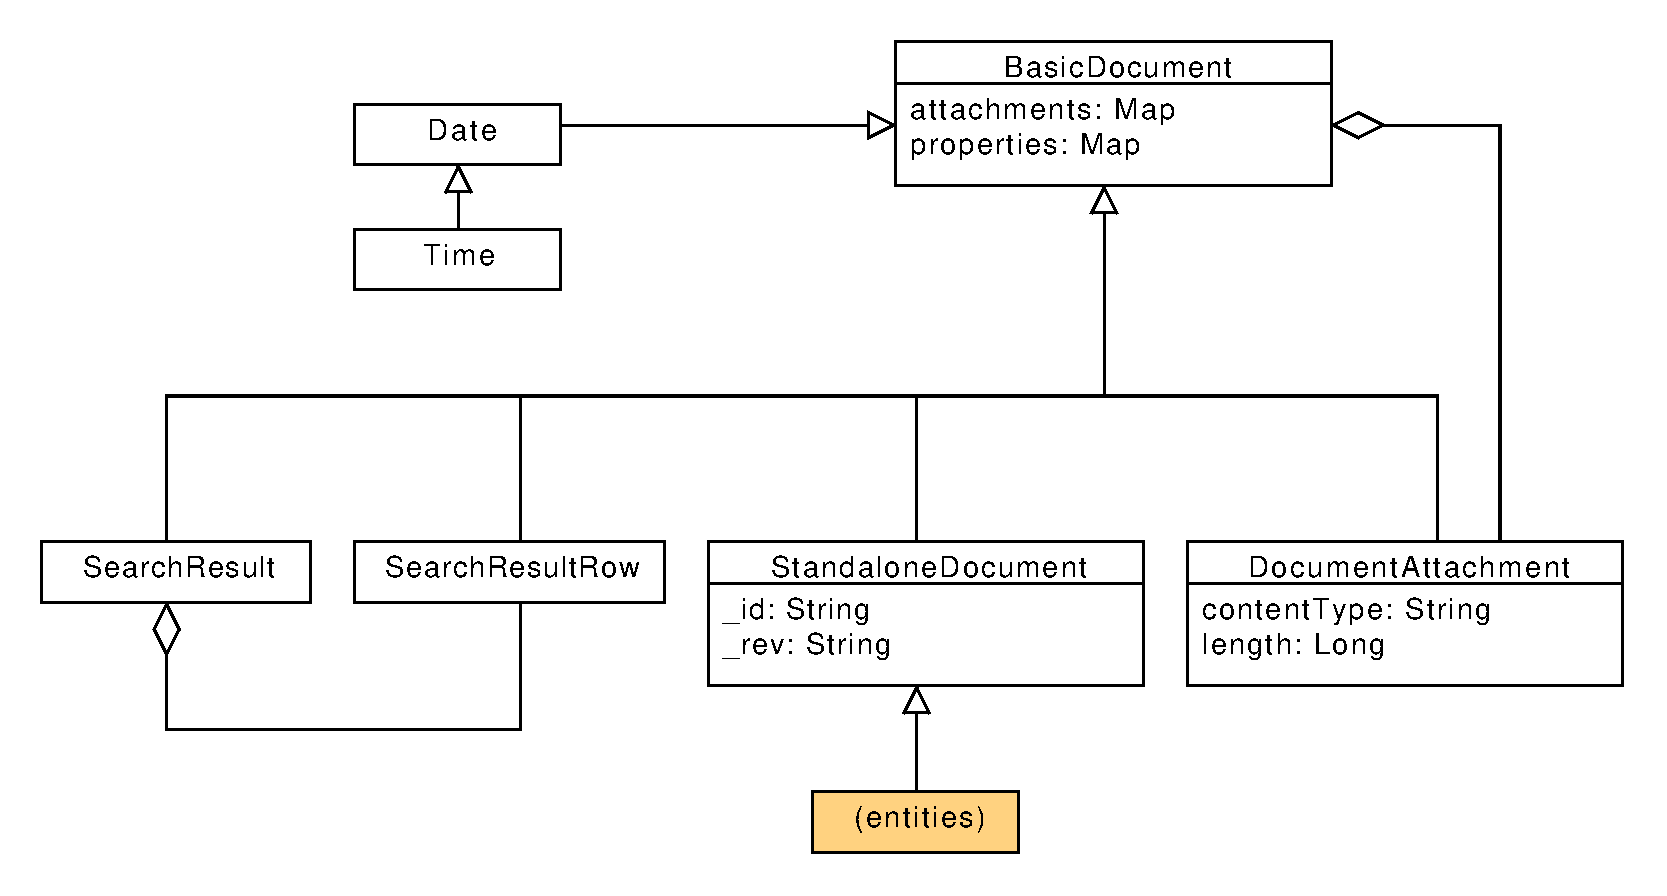
\includegraphics[width=\textwidth]{uml_document.pdf}
\caption{hierarchie dokumentů a entit (UML)}
\label{fig:uml_document}
\end{figure}

\subsubsection{Datový model}

Datový model představuje modelovanou realitu, v tomto případě katalog lístků a podpůrné entity v databázi (uživatele, schránky, komentáře, hlášení, atd.). Jednotlivé složky datového modelu na sobě nejsou přímo závislé, vazby jsou realizovány přes dokumentové ID a jsou tedy typu {\bf String}. Pokud v takové vazbě existuje hodnota {\bf null}, vazba neexistuje. Databáze CouchDB sama žádnou kontrolu integritních omezení neobsahuje, vše obsluhuje datový podsystém aplikace. 

Datový model systému Retrobi je uveden na diagramu~\ref{fig:uml_entity}.

\begin{figure}
\centering
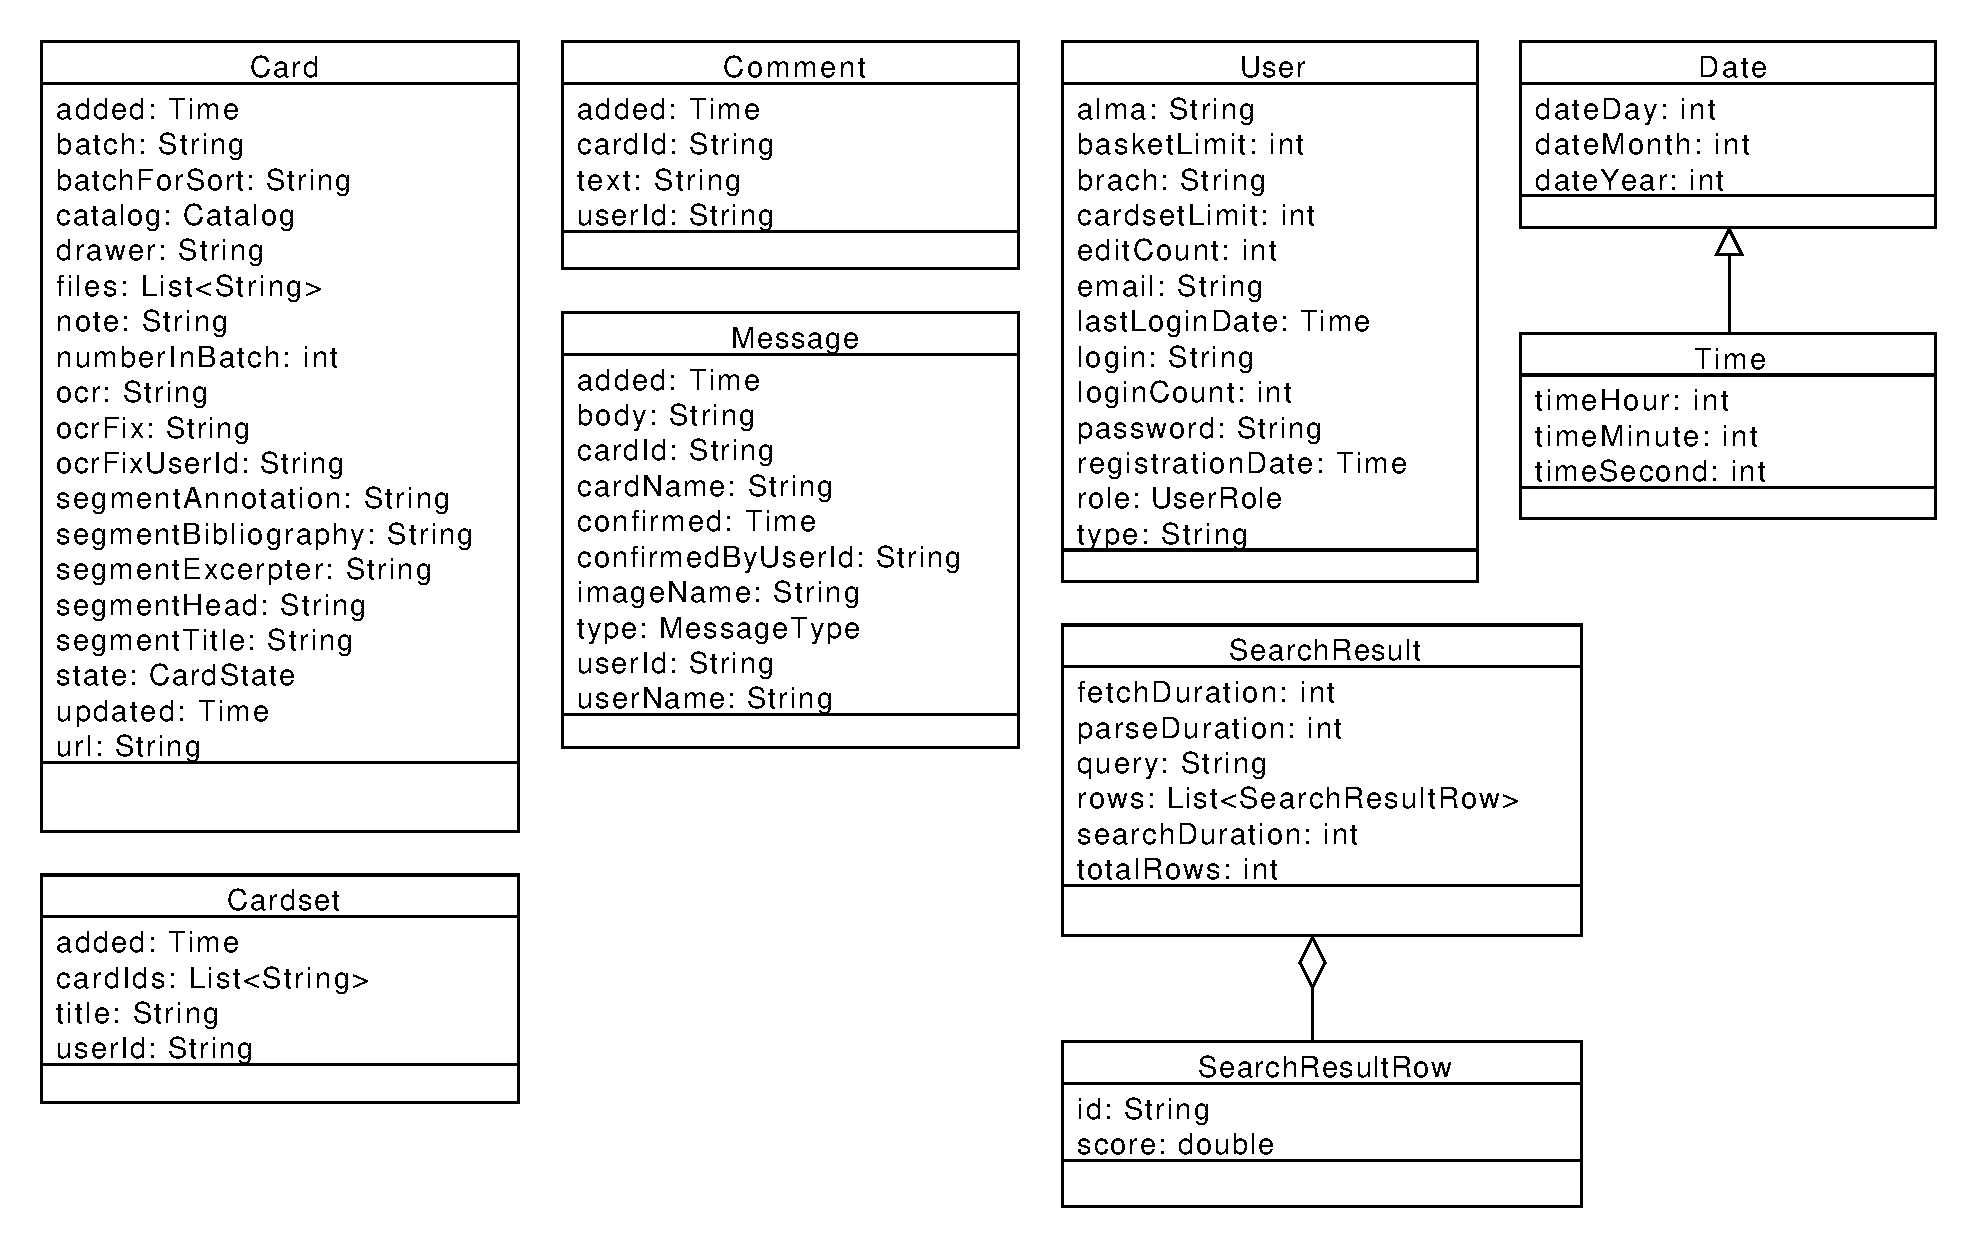
\includegraphics[width=\textwidth]{uml_entity.pdf}
\caption{seznam entit (UML)}
\label{fig:uml_entity}
\end{figure}

Následuje seznam tříd a krátký popis reality, kterou modelují.

\begin{description}
\item[Card:]{lístek (souhrn papírových kartiček a informací na nich obsažených);}
\item[Cardset:]{uložená uživatelská schránka;}
\item[Comment:]{uživatelský komentář k lístku;}
\item[Message:]{hlášení systémové (událost) či uživatelské;}
\item[User:]{registrovaný uživatel;}
\item[SearchResult:]{výsledek vyhledávání;}
\item[SearchResultRow:]{řádek výsledku vyhledávání;}
\item[Date:]{datum (den, měsíc, rok);}
\item[Time:]{datum a čas (den, měsíc, rok, hodina, minuta, sekunda).}
\end{description}

\subsubsection{Stav lístku}

Důležitou vlastností lístku je jeho stav, který vyjadřuje kvalitu a míru přepisu. Prvním a tedy nejnižším stavem je stav \uv{nový}, posledním a tedy nejvyšším stavem je stav \uv{uzavřený}. Každý lístek je v jednom z následujících stavů:

\begin{enumerate}
\item{nový (lístek byl nově uložen do databáze),}
\item{přepsaný (lístek byl editován uživatelem a přepis zatím neprošel redakcí),}
\item{segmentovaný (lístek prošel redakcí a je pro další úpravy uzamčen),}
\item{strukturovaný (lístek obsahuje segmentaci a položkový rozpis),}
\item{uzavřený (lístek je kompletně ověřený, přepsaný a uzavřený).}
\end{enumerate}

\subsubsection{Obrázky lístku}

Obrázky lístku (včetně syntetických) jsou uloženy jako přílohy jednotlivých dokumentů reprezentujících lístky v databázi CouchDB. S těmito přílohami pracuje výhradně repositář {\bf CardImageRepository}, který se stará o jejich načítání, ukládání a mazání. Přílohy dokumentu v databázi CouchDB se nenačítají automaticky s dokumentem samotným kvůli úspoře místa. Proto je načítání obrázků nějakého lístku dodatečná operace.

Každá příloha je jednoznačně daná klíčem (ID) svého rodičovského dokumentu a svým názvem. Název přílohy musí být unikátní v rámci jednoho dokumentu, jinak dochází k nechtěnému přepsání.

\subsubsection{Uživatelské atributy lístku}

Uživatelské atributy lístku je množina hierarchicky uspořádaných hodnot, jejichž struktura se definuje ve zvláštním konfiguračním souboru (viz výše). Tato struktura je po startu systému naparsována a na jejím základě je vytvořen tzv. {\em strom prototypů} (objektů třídy {\bf AttributePrototype}). Každý prototyp se svým okolím je pak předlohou pro jeden či více skutečných atributů (implementujících rozhraní {\bf AttributeNode}). Atributy jsou uspořádány ve stromové struktuře, ve které je každý uzel teoreticky vícenásobný atribut. Atributy jsou buď kompozitní ({\bf ComposedAttributeNode}) s podatributy, nebo atomické ({\bf AtomicAttributeNode}). Atomické atributy (listy stromu) jsou pak nositeli konkrétní řetězcové hodnoty. Strom atributů je přiřazen k lístku.

U každého konkrétního atributu na lístku je možné jednoznačně určit, zda jej lze smazat či klonovat.

Hierarchie atributů a jejich prototypů je uvedena na diagramu~\ref{fig:uml_attribute}.

\begin{figure}
\centering
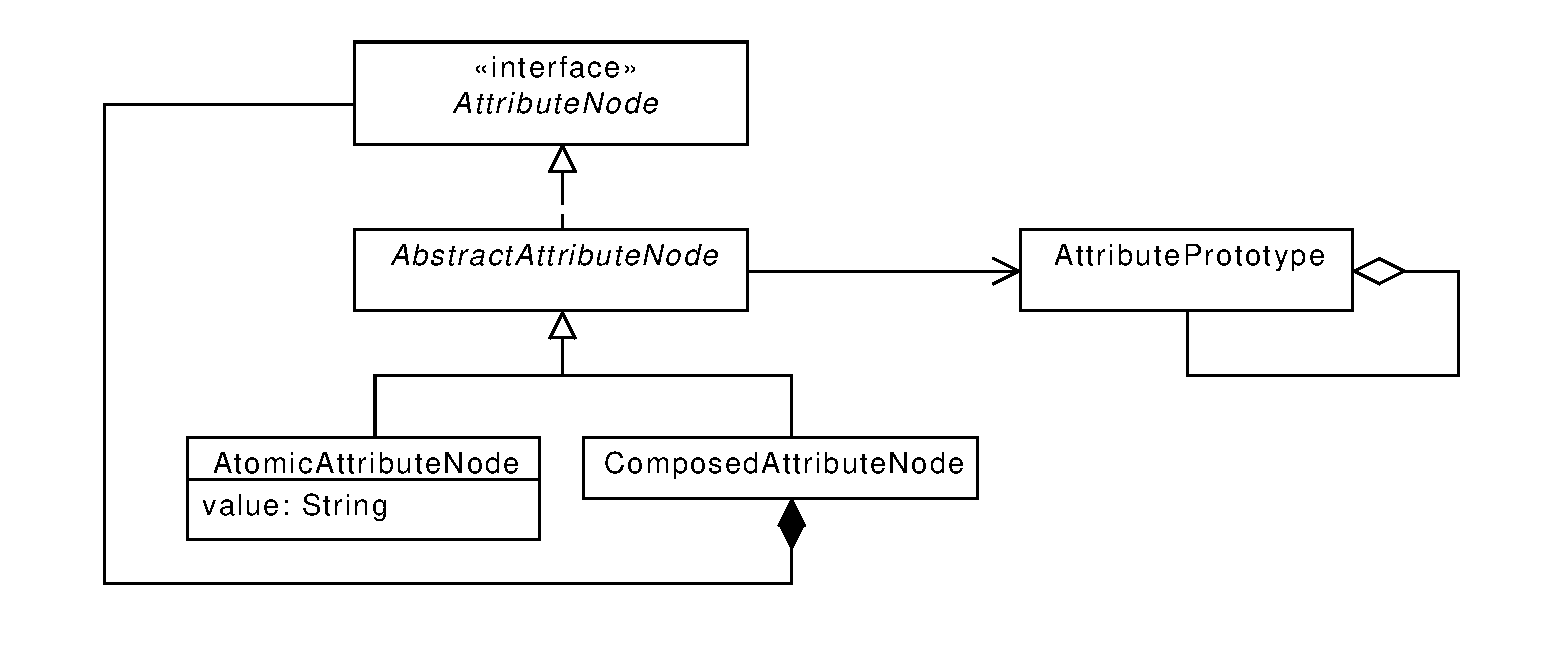
\includegraphics[width=\textwidth]{uml_attribute.pdf}
\caption{atributy lístku (UML)}
\label{fig:uml_attribute}
\end{figure}

\subsubsection{Správa entit v databázi}

Databázový podsystém kromě entit obsahuje i třídy, které se o ně starají, tzv. {\em repositáře}. Repositáře obsahují i definice (kódy Javascript + názvy) souvisejících {\em databázových pohledů}, které slouží jako různé reprezentace dat uložených v databázi CouchDB. Každý repositář spravuje určitou podmnožinu datového modelu.

Základním kamenem repositářů je třída {\bf AbstractProtoRepository}, která obsahuje napojení na knihovnu {\em jcouchdb} a implementuje s její pomocí základní operace CRUD (create, read, update, delete -- vytvořit, načíst, upravit, smazat). Dalším patrem je třída {\bf AbstractRepository}, která od ní dědí. Přidává k ní další a pokročilejší funkce pro dotazování databáze, jako je např. načítání několika entit najednou. Zjednodušuje zkrátka dalším patrům načítání dat a tak zkracuje jejich kód.

Dalšími patry jsou pak již jednotlivé repositáře:

\begin{description}
\item[AnalystRepository:]{analýza lístků v databázi, načítání statistických údajů, rejstřík hodnot;}
\item[CardImageRepository:]{správa obrázků u lístků;}
\item[CardRepository:]{správa lístků a zjišťování struktury katalogu, přečíslování skupin;}
\item[CardSearchRepository:]{spolupráce s vyhledávacím servletem {\em couchdb-lucene} a správa indexů;}
\item[CardsetRepository:]{správa schránek v databázi;}
\item[CommentRepository:]{správa uživatelských komentářů;}
\item[MessageRepository:]{správa uživatelských a systémových hlášení, zápis událostí do CSV logu, záloha a mazání starých hlášení, potvrzování;}
\item[TextRepository:]{správa textů na webu;}
\item[UserRepository:]{správa uživatelů, ověřování přihlašovacích údajů, změna hesla, kontrola duplicitních údajů, žebříček přepisovatelů.}
\end{description}

\begin{figure}
\label{fig:uml_database}
\centering
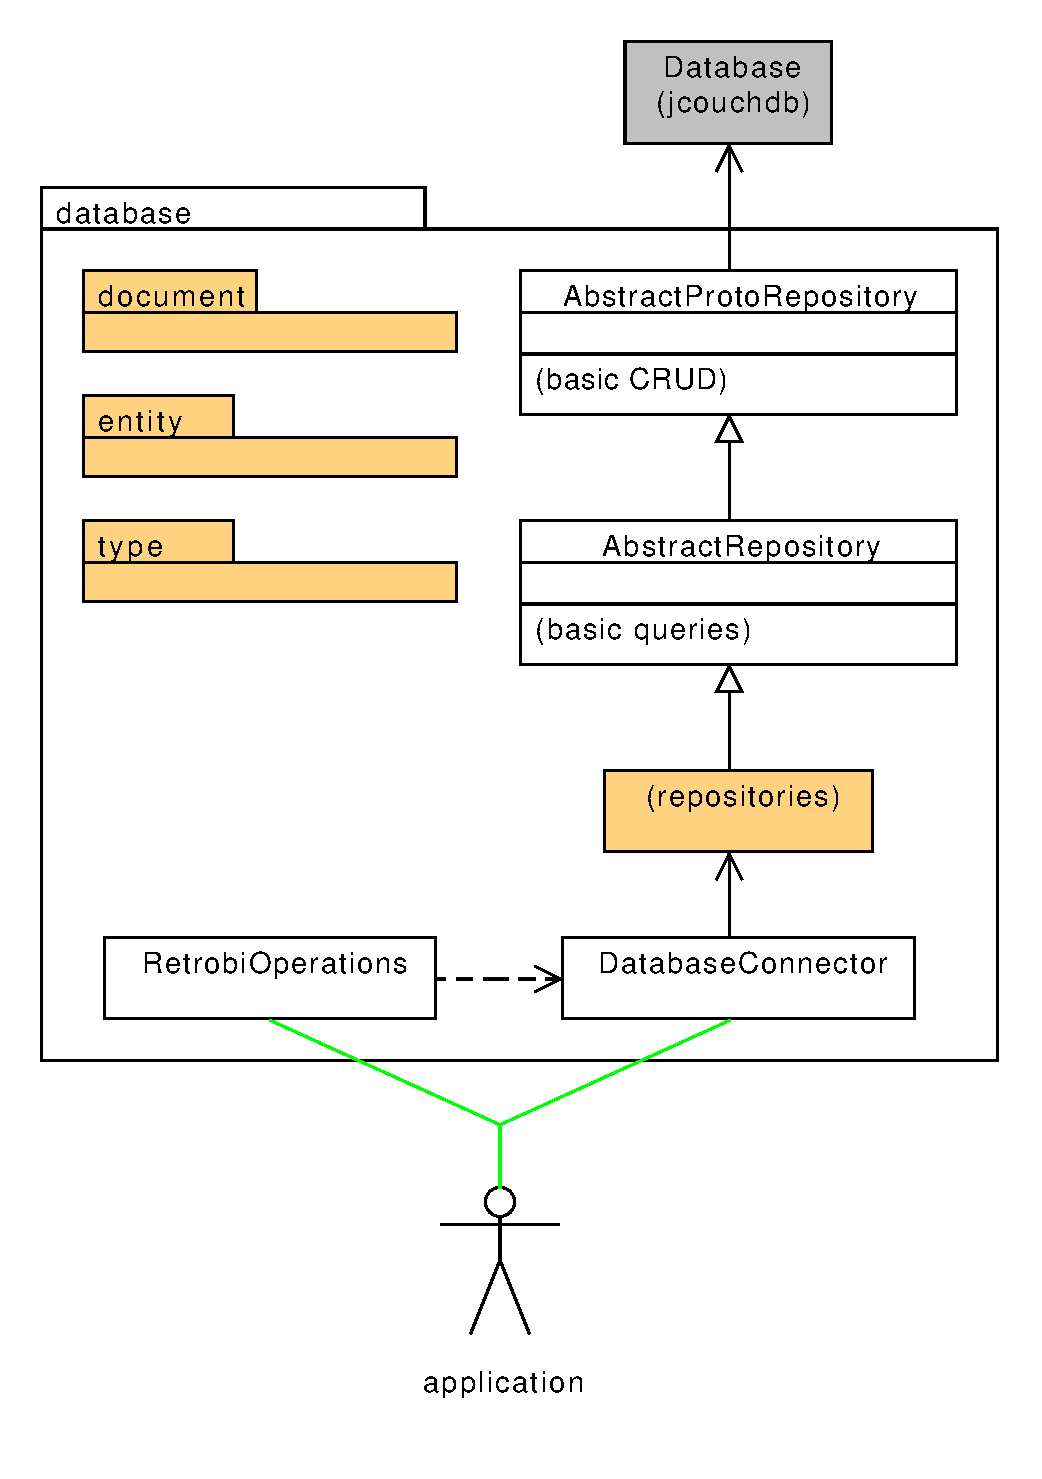
\includegraphics[width=.7\textwidth]{uml_database.pdf}
\caption{správa entit v databázi (UML)}
\end{figure}

Některé operace s entitami v systému Retrobi jsou poměrně komplikované a vyžadují zapojení několika různých repositářů. Takové operace se nachází ve speciální třídě {\bf RetrobiOperations}, která je přístupná ze všech částí aplikace, podobně jako {\bf DatabaseConnector}. Tyto operace jsou:

\begin{description}
\item[Registrace uživatele:]{Před registrací se provede kontrola, zda stejný login či e-mail v databázi již neexistuje. Poté proběhne registrace a nakonec se novému uživateli odešle e-mail s přihlašovacími údaji. Událost se zaloguje.}
\item[Odstranění uživatele:]{Odstraní schránky a komentáře uživatele, poté smaže uživatele, událost se zaloguje a čerstvě odstraněnému uživateli se odešle informační e-mail. Pozor, zde neprobíhá reset uživatelských přepisů, tato funkcionalita je oddělená.}
\item[Změna segmentace:]{Nejdříve se zkontroluje, zda již lístek není uzavřený. Poté se spustí segmentační algoritmus a identifikují se jednotlivé segmenty. Pokud se segmentace povede (nebo je-li segmentace zadána ručně), lístek se v databázi upraví a změna se zaloguje. Poté je stav lístku převeden na \uv{segmentováno}, což je samostatná komplexní operace popsaná níže.}
\item[Změna přepisu OCR:]{Nejdříve se zkontroluje, zda již lístek není uzavřený. Pokud není, k lístku se přiřadí nový přepis včetně autora a lístek je uložen. Událost je zalogována a stav lístku je změněn na \uv{přepsáno}. Změna stavu lístku je samostatná komplexní operace popsaná níže.}
\item[Změna stavu lístku:]{Nejprve je změněn stav lístku a lístek je uložen. Poté se podle minulého a nového stavu rozhodne, které další operace se provedou. Je-li nový stav vyšší než minulý (tzn. lístek má blíže k uzavření), událost se zaloguje a potvrdí se všechna otevřená hlášení u daného lístku. Pokud je nový stav lístku nižší než minulý (tzn. lístek má dále k uzavření), smažou se krycí lístky. V případě, že je nový stav lístku \uv{segmentováno} a vyšší, vytvoří se nové krycí lístky. Hlášení se neukládá, pokud se stav nemění.}
\item[Změna údajů na lístku:]{Lístek je změněn a událost je zalogována. Pokud navíc dojde ke změně poznámky či URL, vytvoří se další události navíc.}
\item[Založení lístku:]{Vytvoří se nový výchozí lístek na zadaném místě a událost se zaloguje.}
\item[Odstranění lístku:]{Odstraní komentáře k danému lístku a potom i vlastní lístek. Událost se zaloguje a skupina je automaticky přečíslována.}
\item[Odstranění přepisů uživatele:]{Nejprve nalezne všechny lístky, které jako poslední přepsal daný uživatel. Reset přepisu se provede u podmnožiny těchto lístků, které mají stav \uv{přepsáno} (reset = smazání přepisu, autora přepisu, celé segmentace a převod stavu lístku na \uv{nový}). Poté se počítadlo přepisů daného uživatele sníží o počet resetovaných lístků.}
\item[Přepnutí stavu potvrzení u hlášení:]{Potvrzené hlášení převede na nepotvrzené a zpět.}
\end{description} 

\subsubsection{Hromadné operace}

Hromadné operace jsou implementovány jako hierarchie tříd implementující rozhraní {\bf CardModification}. Každá tato změna implementuje metodu {\bf modify()}, která obdrží lístek určený k modifikaci, provede úpravu a vrátí logickou hodnotu oznamující, zda úprava proběhla úspěšně, či nikoliv. Fakt, že úprava neproběhla úspěšně, neznamená chybu, ale vznikne při nemožnosti provést změnu nad daným lístkem. Pokud například hromadná operace přidává atribut k lístku, neproběhne úspěšně v případě, že je atribut neopakovatelný a již nějakou hodnotu obsahuje. 

Hromadné operace se dále dělí na obyčejné operace a operace s atributy. Operace s atributy jsou dvě: přidat atribut a odebrat atribut. Obě operace pracují s položkovým rozpisem lístku. Pokud tento neexistuje, je automaticky vytvořen výchozí (dle definice v souboru, viz výše). Operace dědí od abstraktního předka {\bf AbstractAttributeModification}, který zajišťuje načtení a uložení položkového rozpisu před a po konkrétní operaci. 

Všechny hromadné operace mají možnost \uv{odmítnout} úpravu nad konkrétním lístkem -- a to v případě, že lístek zadanou modifikaci {\bf nevyžaduje}. Pokud například nastavujeme novou skupinu lístku, který v této skupině již je, není změna nutná a bylo by zbytečné lístek ukládat a zatěžovat tak bezdůvodně databázi. Z tohoto důvodu může metoda {\bf modify()} skončit s výjimkou {\bf AlreadyModifiedException}, kterou nadřazená vrstva zachytí a lístek přeskočí.

\begin{figure}
\label{fig:uml_modify}
\centering
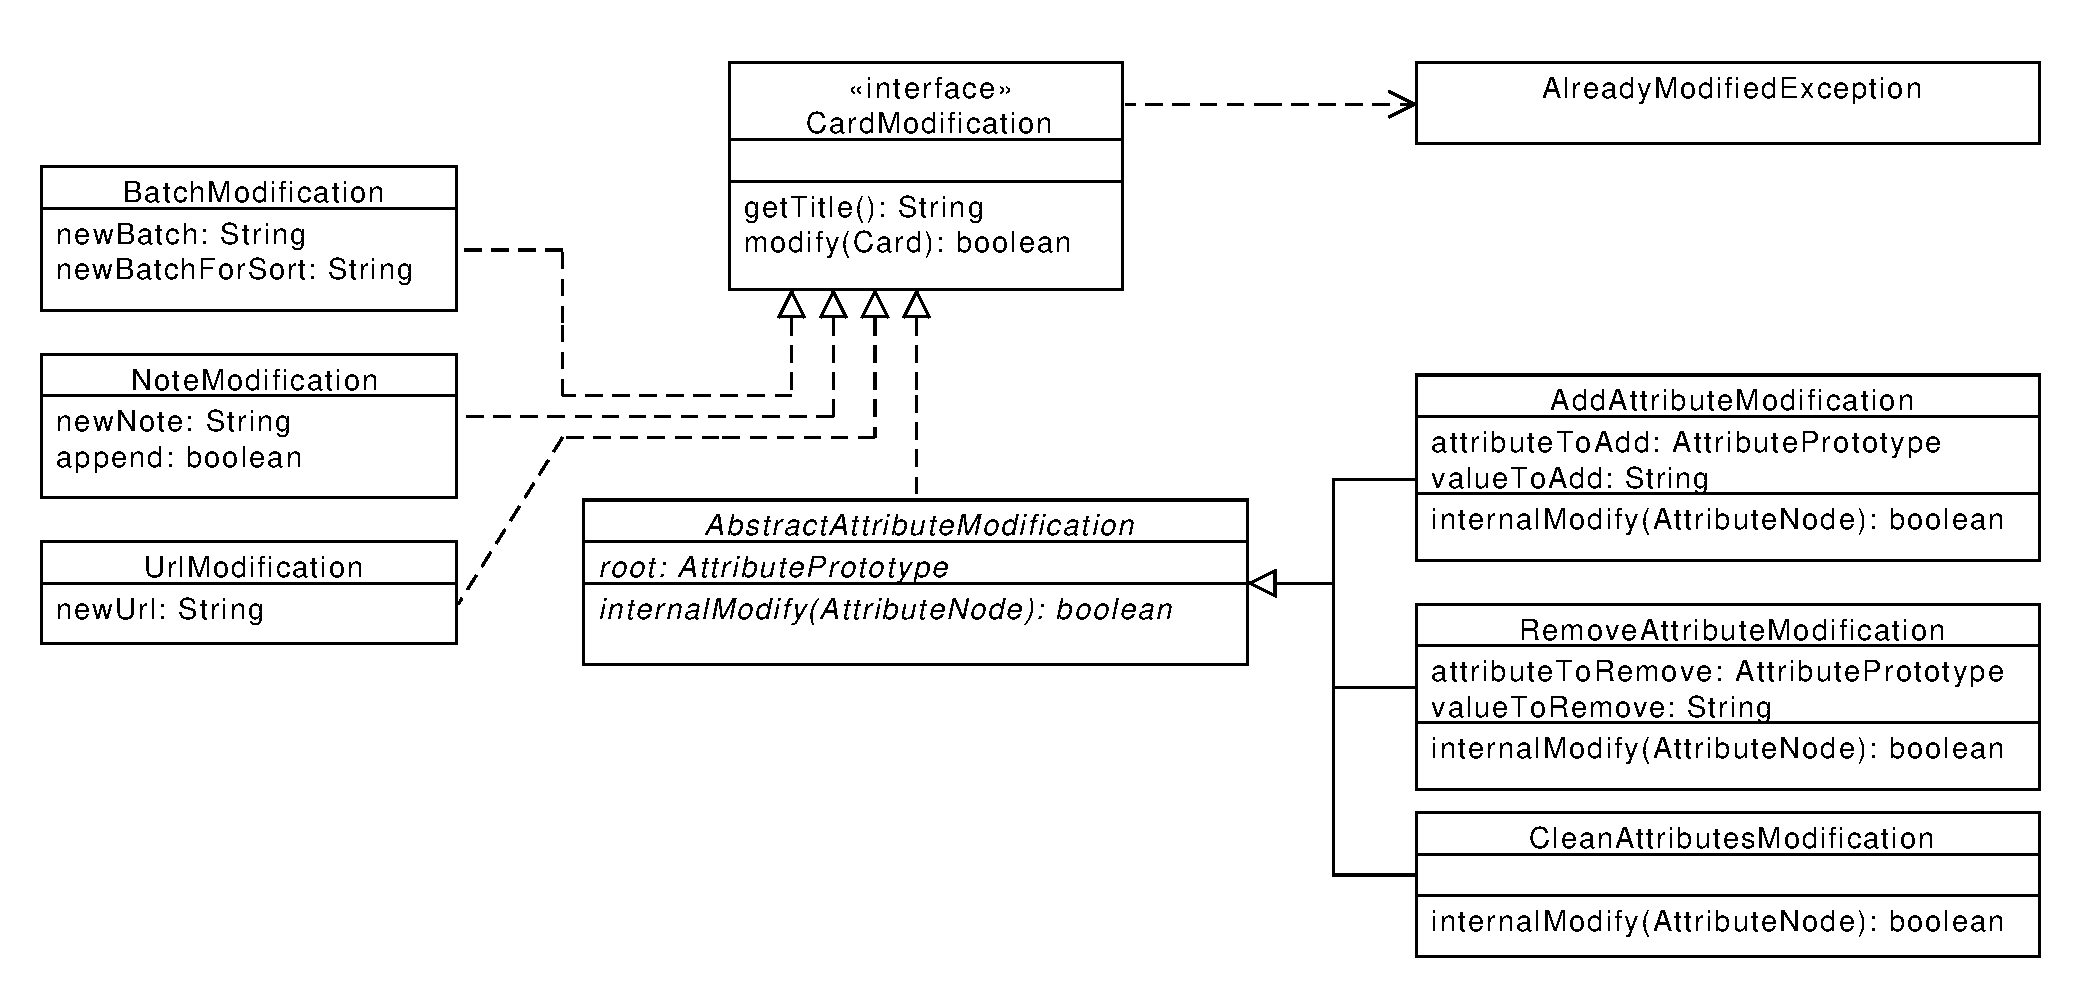
\includegraphics[width=\textwidth]{uml_modify.pdf}
\caption{hromadné operace nad lístky (UML)}
\end{figure}

\subsubsection{Vyhledávání}

Pro vyhledávání je použita univerzální platforma Lucene od nadace Apache. Tato platforma je podobně jako CouchDB založena na dokumentech, ale mezi dokumenty CouchDB a Lucene je nutný určitý netriviální převod. Hodnoty uložené v indexu se totiž mohou lišit od hodnot v databázi. Vše záleží na definici indexů -- některé indexy mohou obsahovat jen přepis OCR, jiné zase skupiny, atd. 

Tvorbu a obsluhu indexů zajišťuje servlet CouchDB Lucene, který je neustále spuštěný a očekává požadavky na samostatném portu. 

Databáze CouchDB je nastavena tak, že hlásí všechny změny tomuto indexovacímu servletu a ten svůj index postupně aktualizuje. Platforma Lucene tedy není využita přímo, ale přes zmíněný servlet. Vyhledávání je na databázi nezávislé a vyhledávání jako takové nezatěžuje databázi, jen samotný indexovací server (za předpokladu, že jsou servery fyzicky oddělené).

Vyhledávací dotaz se (podobně jako dotazy databázové) spustí požadavkem na určitou URL adresu, na které vyhledávací servlet poslouchá. Jako parametr je v ní specifikován uživatelský dotaz, název indexu a také název pole, ve kterém se má hledání provést. Lucene podporuje širokou škálu různých vyhledávacích technik, například fuzzy dotaz, kombinovaný dotaz, dotaz na číselný rozsah, použití divokých karet a další.

Výsledky vyhledávání jsou pak předány zpět webové aplikaci, která dotaz spustila, a obsahují metainformace (čas vyhledávání, čas načítání, celkový počet výsledků bez stránkování) a řádky, ve kterých je klíčová hodnota ID obsahující ID nalezeného dokumentu a související hodnoty. V těchto hodnotách pak lze provést zvýraznění výsledků.

\subsubsection{Společné knihovny}

Společná knihovna metod je skupina několika nezávislých tříd, které obsahují různé užitečné statické metody. Každá třída realizuje určitý okruh funkcionalit a zpravidla jsou k ní napsány unit testy, které ověřují korektnost metod. Následuje seznam těchto tříd se stručným popisem jejich zodpovědnosti:

\begin{description}
\item[DefaultAttributePrototyper:]{Vytváří výchozí definici položkového rozpisu (stromu atributů) a indexů, pokud nejsou nalezeny žádné uživatelsky definované.}
\item[SimpleAttributeUtils:]{Pracuje s položkovým rozpisem -- vyhledává, přidává a odebírá atributy, podporuje import a export struktury do souboru a získání i vložení vyplněné struktury do dokumentu.}
\item[SimpleDatabaseUtils:]{Zajišťuje vytvoření design dokumentu zadaných repositářů v databázi a obsahuje metody pro práci s identifikátory ({\bf \_id}) design dokumentů.}
\item[SimpleExportUtils:]{Obsahuje metody pro export lístků do RTF a ZIP.}
\item[SimpleFileUtils:]{Obsahuje metody pro práci se soubory -- extrahování různých informací z jejich názvů, jejich načítání a zápis, validaci, přesun a kopírování.}
\item[SimpleFrameUtils:]{Obsahuje metody pro zobrazení různých dialogů: potvrzení, zpráva, chybové hlášení a výběr souboru.}
\item[SimpleGeneralUtils:]{Obecné metody pro práci s objekty a jejich kolekcemi. Obsahuje i poměrně důležitý algoritmus pro přesun objektu v rámci nějaké kolekce.}
\item[SimpleImageUtils:]{Klíčová knihovna pro práci s obrázky. Obsahuje metody pro načítání a zápis obrázků, jejich konverzi, vytváření náhledů, škrtání, otočení, detekci prázdných stran a generování syntetických obrázků.}
\item[SimpleIndexUtils:]{Obsahuje jen jednu veřejnou metodu pro vytvoření vyhledávacích indexů. Tato funkce je ale natolik složitá a zároveň ostře ohraničená, že byla přesunuta do vlastní třídy.}
\item[SimpleSearchUtils:]{Obsahuje pomocné metody pro získávání seznamu lístků z výsledku vyhledávání, pro zvýrazňování hledaných výrazů ve fragmentech a pro normalizaci vyhledávacího dotazu.}
\item[SimpleSegmentUtils:]{Obsahuje segmentační algoritmus a metody pro extrakci jednotlivých segmentů dle určených formátovacích pravidel z přepisu obsahujícího segmentační znaky. Také převádí lístky do textové reprezentace, která se využívá v různých částech webové aplikace.}
\item[SimpleStringUtils:]{Knihovna metod pro práci s řetězci, která patří mezi ty nejrozsáhlejší. Obsahuje metody pro kódování a dekódování (base64, hashe, CSV, JSON), získávání náhodného řetězce, skloňování, validaci, typografickou opravu, zalamování řádků a různé netriviální úpravy řetězce. Také obsahuje různé malé sémantické funkce pro zjednodušení kódu webové části.}
\end{description}

\subsubsection{Vyhledávání}

O vyhledávání se stará třída {\bf CardSearchRepository}, která posílá správné požadavky na vyhledávací servlet CouchDB-Lucene. Takový požadavek může vypadat například takto:

\begin{verbatim}
/retrobi/_fti/_design/index/basic_ocr_best
?allow_leading_wildcard=true&lowercase_expanded_terms=true
&qsplit=false&skip=0&limit=1
&q=%2Bdefault_lc%3A%28*psac%C3%AD*+%2B+*stroj*+%281870+to+1920%29%29
\end{verbatim}

Tento dotaz byl zavolán na indexu {\bf basic\_ocr\_best} (nejlepší dostupný textový přepis) a jedná se o dotaz necitlivý na velikost písmen. Z výsledků bude vybrán jen první lístek (skip = 0, limit = 1). Dotaz je \uv{*psací* *stroj* [1870 TO 1920]}.

\subsubsection{Rozsah lístků}

Rozsah lístků je zde chápán jako interval lístků v katalogu. Tento interval může být libovolně velký, vždy je však nutné z něj vybrat několik {\em reprezentantů}, podle kterých se uživatel bude orientovat a rozsah měnit. To si můžeme představit jako listování šuplíkem, který si rozdělíme např. na deset stejně velkých částí. Pak se podíváme na první lístek každé části a tak zjistíme, ve které části najdeme lístek požadovaný. 

Rozsah lístků se používá při procházení katalogu (část / skupina), ale i schránky a výsledků vyhledávání. U výsledků vyhledávání je ale rozsah omezen pouze na jednotlivé lístky (z výkonnostních důvodů).

K reprezentaci rozsah lístku nestačí dvě čísla (offset a limit), jak je zvykem v běžných stránkovacích aplikacích. Může totiž existovat i poměrně velký rozsah lístků, ze kterého je viditelných jen několik reprezentativních lístků. Například pro rozsah 1--1000 a počet lístků 10 jsou viditelné lístky 1, 101, 201, 301, \ldots, 901. Rozsah tedy musí obsahovat informaci, kolik lístků má načíst celkem, z čehož dopočítá, kolik lístků se musí pokaždé přeskočit.

Pro ilustraci uvádíme v tabulce~\ref{tab:range} několik příkladů. V každém řádku tabulky jsou tři vstupní údaje: počet lístků, číslo prvního lístku a velikost skoku mezi dvěma reprezentanty. Za nimi jsou v řádku uvedené čísla reprezentantů a odpovídající rozsahy. Každý viditelný lístek tedy vlastně reprezentuje další rozsah lístků (až do úrovně jednotlivých lístků, kdy každý lístek reprezentuje právě sám sebe).

\begin{table}
\begin{center}
\begin{tabular}{|c|c|c|p{5cm}|p{5cm}|}
\hline
Počet lístků & První & Skok & = Reprezentanti & = Rozsahy \\
\hline
\hline
54 & 1 & 10 & 1, 11, 21, 31, 41, 51 & 1--10, 11--20, 21--30, 31--40, 41--50, 51--54 \\
\hline
54 & 7 & 10 & 7, 17, 27, 37, 47 & 7--16, 17--26, 27--36, 37--46, 47--54 \\
\hline
842 & 3 & 100 & 3, 103, 203, 303, 403, 503, 603, 703, 803 & 3--102, 103--202, 203--302, 303--402, 403--502, 503--602, 603--702, 703--802, 803--842 \\
\hline
842 & 1 & 1000 & 1 & 1--842 \\
\hline
842 & 124 & 1000 & 124 & 124--842 \\
\hline
4321 & 7 & 1000 & 7, 1007, 2007, 3007, 4007 & 7--1006, 1007--2006, 2007--3006, 3007--4006, 4007--4321 \\
\hline
\end{tabular}
\end{center}
\caption{příklady rozsahů (intervalů) lístků a jejich reprezentantů}
\label{tab:range}
\end{table}

Z tabulky~\ref{tab:range} vyplývají výpočty a různé způsoby reprezentace rozsahů.

Rozsah lístků je reprezentován dvěma {\em neměnnými} (konstantními) třídami: {\bf CardRange} a {\bf CardCatalogRange}. První z nich reprezentuje obecný rozsah, zatímco ta druhá rozsah v určitém katalogu a skupině. Druhá třída je postavena na první, a tak je dostačující věnovat se jí.

Třída {\bf CardRange} obsahuje následující stavové proměnné, které se nikdy nemění (při změně zobrazeného intervalu je vždy vytvořen na základě starého intervalu nový):

\begin{description}
\item[count:]{celkový počet lístků v procházené podmnožině (ne v celém katalogu);}
\item[offset:]{počáteční offset intervalu (přesah), tedy číslo prvního lístku bez jedné (přesah je číslován od 0, lístky od 1);}
\item[range:]{velikost intervalu, tedy počet lístků reprezentovaných tímto intervalem (např. pro lístky 1--99 má hodnotu 100);}
\item[bigstep:]{počet reprezentantů, tedy počet najednou zobrazených lístků (tato hodnota ovlivňuje i počet a členitost stromu intervalů);}
\item[flat:]{příznak plochého intervalu s jednou úrovní -- pokud je příznak platný, neexistuje vyšší ani nižší interval, pohybovat se lze jen vlevo a vpravo;}
\item[type:]{typ intervalu (pouze pro zobrazení správné \uv{šipky}).}
\end{description}

Dále obsahuje tovární metody pro vytváření dalších intervalů:

\begin{description}
\item[createFirst():]{interval obsahující jen první lístek;}
\item[createLast():]{interval obsahující jen poslední lístek;}
\item[createNext():]{následující interval na stejné úrovni;}
\item[createPrevious():]{předchozí interval na stejné úrovni;}
\item[createLower(int):]{nižší interval (parametr určuje který);}
\item[createUpper():]{vyšší interval;}
\item[createForOtherCount(int):]{podobný interval pro jiný počet lístků.}
\end{description}

Tovární metody vytváří na základě aktuálního intervalu jiné intervaly, které zachovávají jeho základní nastavení, tedy počet reprezentantů a celkový počet lístků. Při změně počtu reprezentantů nebo lístků se musí vytvořit nový základní interval, který bude tento počet respektovat, a to i v dalších jím vytvořených intervalech.

Příklad ilustruje obrázek~\ref{fig:range}.

\begin{figure}
\centering
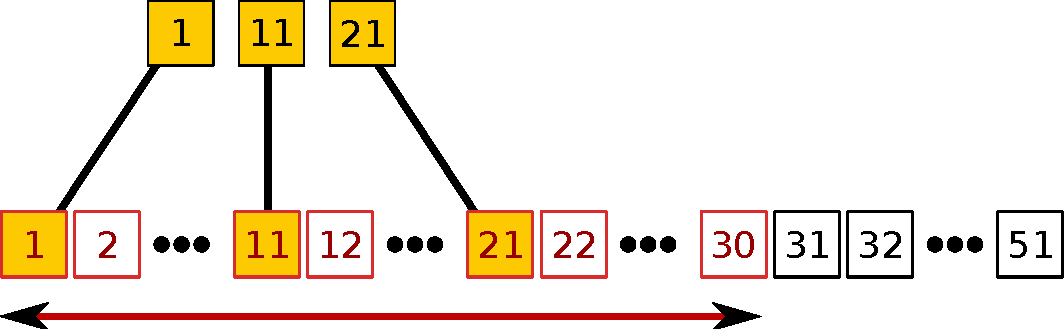
\includegraphics[width=.7\textwidth]{range.pdf}
\caption{ilustrace k rozsahu lístků: počet lístků = 51, počet reprezentantů = 3, interval = 1--30, výslední reprezentanti = 1,~11,~21}
\label{fig:range}
\end{figure}

\subsubsection{Ostatní třídy}

\begin{description}
\item[RetrobiLocker:]{Objekt obsahující rozličné zámky, na kterých probíhá synchronizace skupin proměnných.}
\item[CSVHistoryLogger:]{Třída, která zapisuje data ve formátu CSV do souboru, jehož jméno je dáno aktuálním datumem. Druhého ledna roku 2000 bude například zápis probíhat do souboru {\bf 2000-01-02.csv}. Tato třída slouží k průběžnému logování důležitých operací systému.}
\item[CzechAlphabet:]{Třída obsahující českou abecedu a metody pro řazení řetězců. Také zahrnuje funkcionalitu pro získávání prvního písmene skupiny a generování výchozí skupiny pro řazení.}
\item[DataLoader:]{Rozhraní objektu, který dokáže načíst uspořádanou podmnožinu položek zadané maximální velikosti od určité pozice. Tento objekt se používá ve spolupráci s třídou {\bf CardRange}, která jej umí využít jako zdroj dat k získání reprezentantů, tedy např. lístků z intervalu.}
\item[DataToExport:]{Nastaví exportu schránky.}
\item[Triple:]{Uspořádaná trojice.}
\item[Tuple:]{Uspořádaná dvojice.}
\end{description}

\subsubsection{Systémová hlášení}

Systémovým hlášením se v systému Retrobi rozumí speciální záznam v databázi. Tento záznam je reprezentován entitou {\bf Message} a jeho nejdůležitějšími vlastnostmi je datum vložení, typ, obsah a potvrzení. Typ hlášení nabývá hodnot ze dvou kategorií: systémové události (events) a hlášení o problémech (problems). Systémové události přidává systém sám, zatímco hlášení o problémech jsou přidávána ručně uživateli. Administrátor může tato hlášení prohlížet ve Správě a potvrzovat ty, které vzal na vědomí, případně vyřešil.

V této části dokumentace se budeme zabývat jen systémovými událostmi. Existují tyto druhy systémových událostí:

\begin{description}
\item[EVENT\_BATCH\_UPDATED:]{Změna skupiny.}
\item[EVENT\_OCR\_UPDATED:]{Změna OCR.}
\item[EVENT\_SEGMENTS\_UPDATED:]{Změna segmentace.}
\item[EVENT\_NOTE\_UPDATED:]{Změna poznámky.}
\item[EVENT\_URL\_UPDATED:]{Změna URL.}
\item[EVENT\_STATE\_UPDATED:]{Změna stavu lístku.}
\item[EVENT\_CARD\_CREATED:]{Lístek založen.}
\item[EVENT\_CARD\_REMOVED:]{Lístek smazán.}
\item[EVENT\_CARD\_MODIFIED:]{Hromadná operace.}
\item[EVENT\_MULTIPLE\_CARDS\_MODIFIED:]{Hromadná operace (více lístků).}
\item[EVENT\_CARD\_MOVED:]{Hromadný přesun.}
\item[EVENT\_MULTIPLE\_CARDS\_MOVED:]{Hromadný přesun (více lístků).}
\item[EVENT\_USER\_REGISTERED:]{Registrace uživatele.}
\item[EVENT\_USER\_REMOVED:]{Uživatel smazán.}
\item[EVENT\_IMAGE\_CROSS\_ON:]{Zaškrtnutí lístku.}
\item[EVENT\_IMAGE\_CROSS\_OFF:]{Zrušeno zaškrtnutí lístku.}
\end{description}

Všechna hlášení se ukládají jako nepotvrzená až na několik výjimek. Hlášení o změně segmentace (EVENT\_SEGMENTS\_UPDATED) se po vložení automaticky uzávírá právě tehdy když je stav lístku vyšší než Přepsáno (REWRITTEN), tedy segmentováno a výše. Hlášení o změně stavu (EVENT\_STATE\_UPDATED) se uzavírá právě tehdy když je nový stav lístku vyšší než původní stav a zároveň je přihlášen editor či vyšší.

\subsection{Jednoúčelové nástroje}

\begin{figure}
\label{fig:uml_tools}
\centering
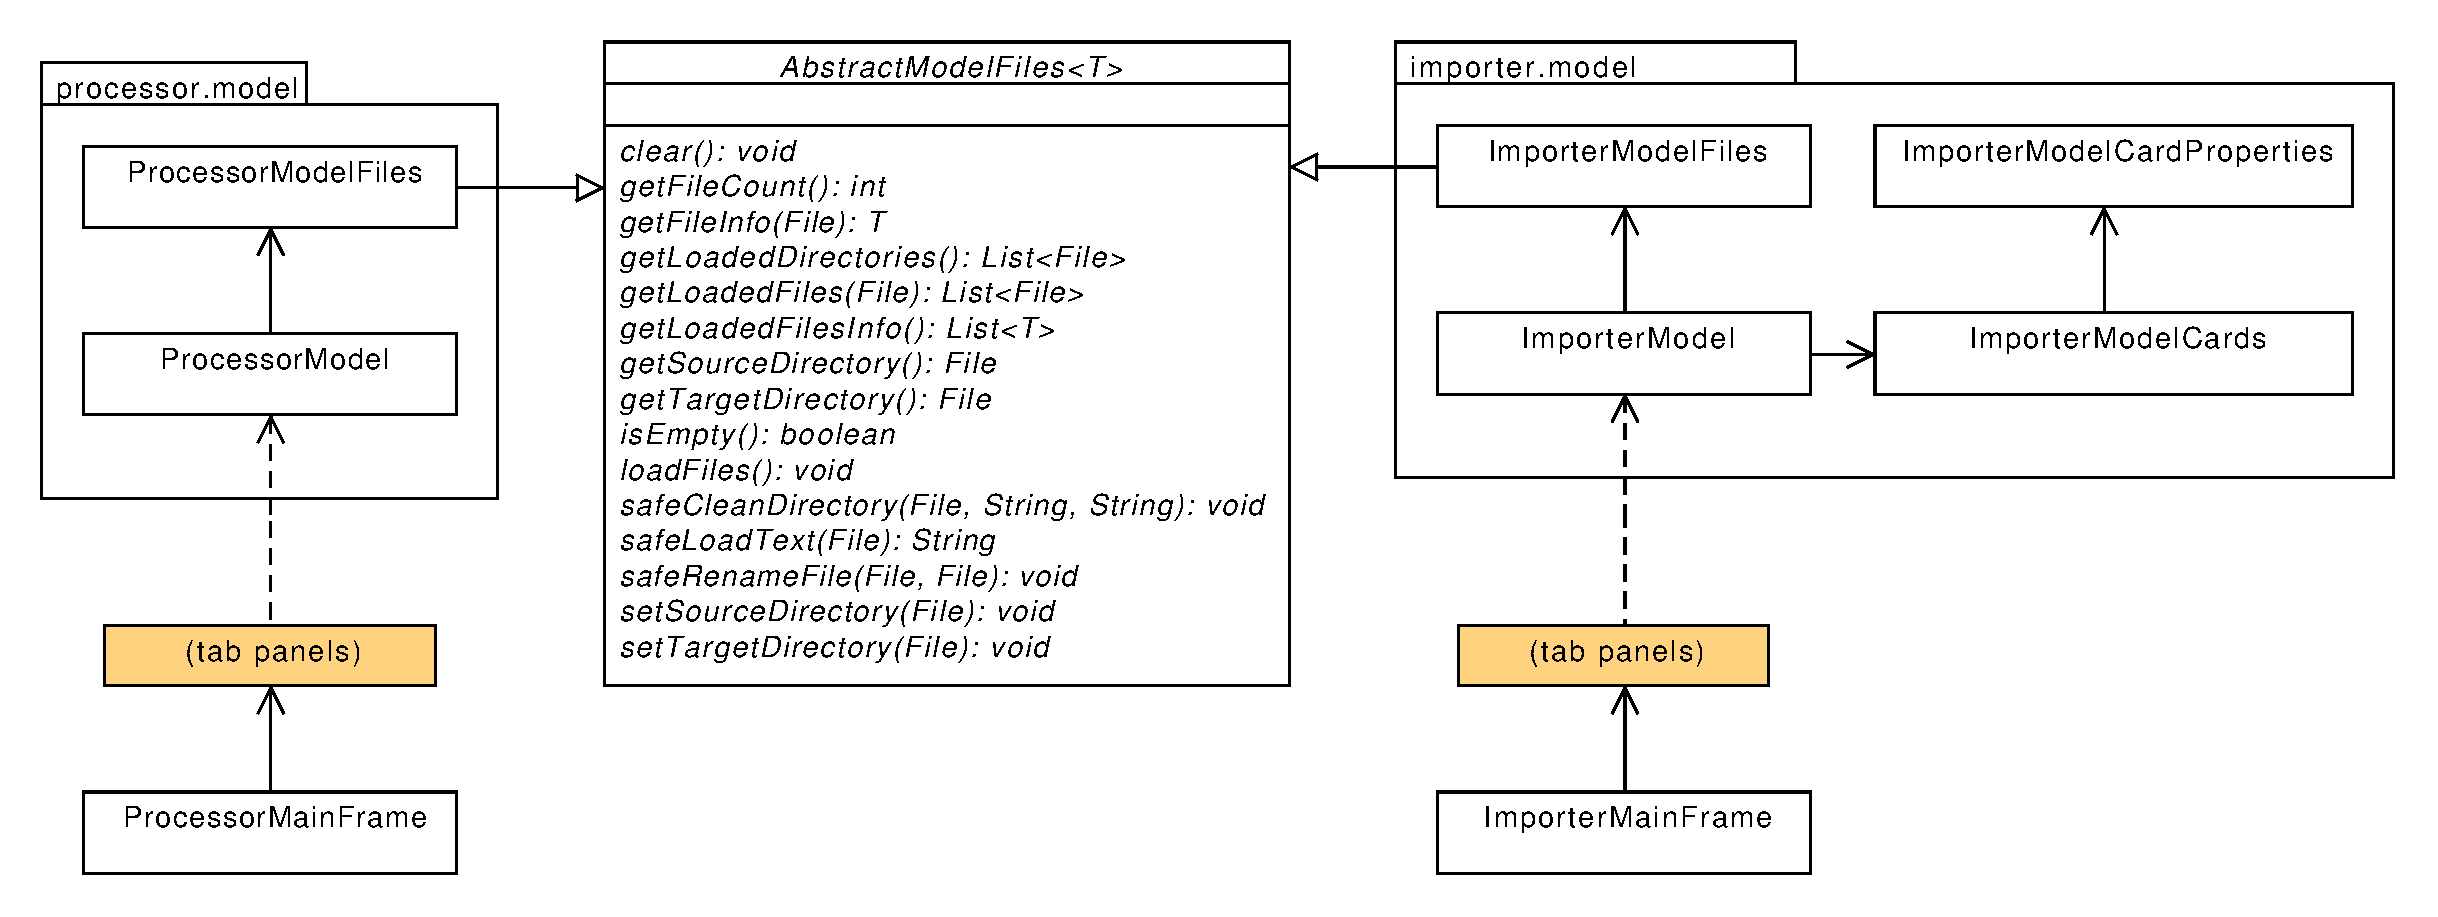
\includegraphics[width=\textwidth]{uml_tools.pdf}
\caption{základní struktura nástrojů (UML)}
\end{figure}

\begin{figure}
\label{fig:uml_files}
\centering
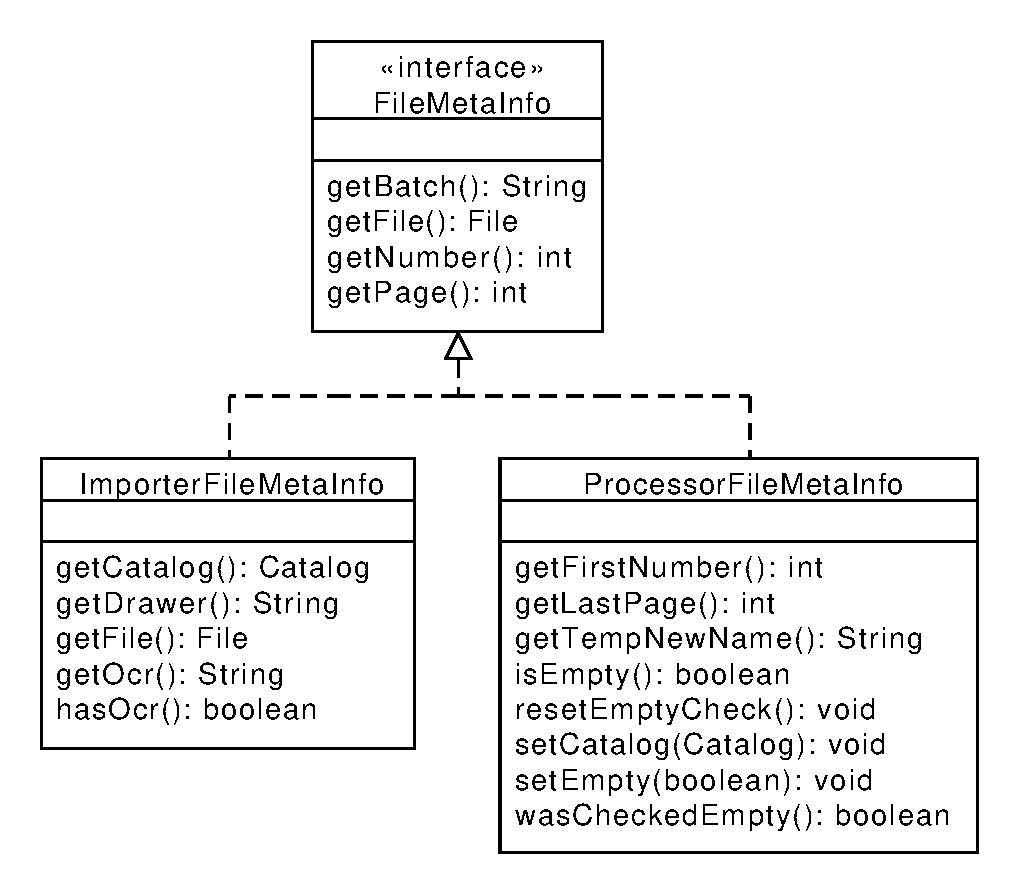
\includegraphics[width=.5\textwidth]{uml_files.pdf}
\caption{hierarchie metasouborů (UML)}
\end{figure}

Systém Retrobi obsahuje dva nástroje pro zpracování a import naskenovaných dat do databáze. Technicky jsou zde označeny jako {\em processor} (přejmenování, konverze, detekce prázdných stran lístků) a {\em importer} (zmenšení, zařazení, upload zpracovaných obrázků). Spouštějí se přes webové rozhraní (v sekci {\em Správa / Nástroje}). Technicky vzato je lze spustit i ručně ze zkompilovaného JARu ({\em retrobi-tools.jar}), ale nedoporučuje se to - spuštění přes webové rozhraní (technologie JNLP) totiž doplní jejich konfigurační parametry, což při manuálním spuštění chybí.

Oba nástroje (procesor i importer) pracují především s obrázkovými soubory. Proto oba obsahují kolekce pro uchování těchto souborů ({\bf ProcessorModelFiles}, {\bf ImporterModelFiles}). Společná či zobecněná funkcionalita shrnuta ve společném předkovi {\bf AbstractModelFiles}. Tento předek uchovává soubory spolu s meta-informacemi ({\bf ProcessorFileMetaInfo}, {\bf ImporterFileMetaInfo}), které jsou extrahovány po načtení nové sady souborů. Oba nástroje obsahují hlavní model, který se dále dělí na podmodely. Model poskytuje funkcionalitu a data nad ním postavenému grafickému rozhraní. Následuje detailnější popis obou modelů.

U procesoru neexistuje spojení s databází a vše se děje na úrovni souborů (např. přejmenování, přesun, detekce prázdných stránek, konverze). Proto je jeho model jednodušší a obsahuje pouze kolekci souborů. 

U importeru existuje spojení s databází a z obrázkových souborů se vytváří lístky. Proto je jeho model rozdělen na kolekci souborů ({\bf ImporterModelFiles}) a a kolekci lístků ({\bf ImporterModelCards}). Kolekce lístků dále obsahuje model pro tvorbu a uchování jejich vlastností ({\bf ImporterModelCardProperties}). 

Oba nástroje svou činnost logují do souboru CSV.

\subsubsection{Detekce prázdných stránek}

Detekce prázdných stránek v aplikaci Retrobi není nic složitého, jen aplikace středoškolské statistiky a několik jednoduchých nápadů. Provádí se jednou, a to při zpracování lístku po skenování. Detekce se skládá z těchto kroků:

\begin{enumerate}
\item{Z obrázku se vytvoří menší náhled, aby zpracování netrvalo tak dlouho.}
\item{Oříznou se hrany, které mohou obsahovat nepřesné, pomačkané či špinavé okraje lístku. Tím se zvýší účinnost rozpoznávání.}
\item{Z tohoto fragmentu se vypočítá barva papíru (barva, jejíž složky jsou mediány odpovídajících barevných složek všech pixelů -- algoritmus: do tří polí se postupně uloží barevné složky všech pixelů, pole se seřadí a z každého se vezme prostřední prvek).}
\item{Vypočítá se světelnost barvy papíru (0.3 * r + 0.59 * g + 0.11 * b).}
\item{Světelnost barvy papíru se vynásobí malou konstantou a vyjde prahová světelnost, tedy nejvyšší světelnost, kterou může mít inkoust na daném lístku.}
\item{Spočítá se, kolik pixelů má podprahovou světelnost (= kolik inkoustu tam je).}
\item{Pokud relativní počet tmavých pixelů přeroste určitou mez, je lístek označen jako neprázdný, jinak je považován za prázdný.}
\end{enumerate}

Během procesu je použito několik parametrů, které byly náhodným testováním vyladěny tak, aby detekce dávala co nejlepší výsledky na testované množině.

\subsection{Webová aplikace}

Webová aplikace je postavena na frameworku {\em Wicket}. Nejprve zde stručně popíšeme základní rysy frameworku a způsob, jakým jsou v něm generovány stránky. Domovská stránka frameworku {\em Wicket} je {\bf http://wicket.apache.org/}, kde se nachází dokumentace a příklady použití. 

Hlavní třída webové aplikace systému Retrobi se jmenuje {\bf RetrobiWebApplication}. Tato třída dědí od třídy {\bf WebApplication} specifikované ve frameworku Wicket a je jakýmsi vstupním bodem do celého webového podsystému. Spravuje vytváření a obsluhu webových požadavků, řídí ukládání uživatelských relací (sessions), spouští dlouhé úlohy, pravidelně spouští systémovou údržbu a obsahuje názvy všech parametrů URL. Také se zde při spuštění aplikace (metoda {\bf init()} inicializují všechny parametry frameworku Wicket tak, aby jeho chování odpovídalo požadavkům systému Retrobi. Při startu aplikace napsané nad frameworkem Wicket se také připojují všechny {\em zdroje}, což jsou v případě systému Retrobi soubory JNLP pro spuštění jednorázových importovacích nástrojů (tzv. \uv{udělátek}, zdroj implementován třídou {\bf JnlpResource}) a obrázky jednotlivých lístků (zdroj implementován třídou {\bf CardImageResource}). Podobně se mapují i jednotlivé webové stránky -- ke každé stránce je připojena \uv{lidová} adresa, na které ji lze najít.

\begin{figure}
\label{fig:uml_application}
\centering
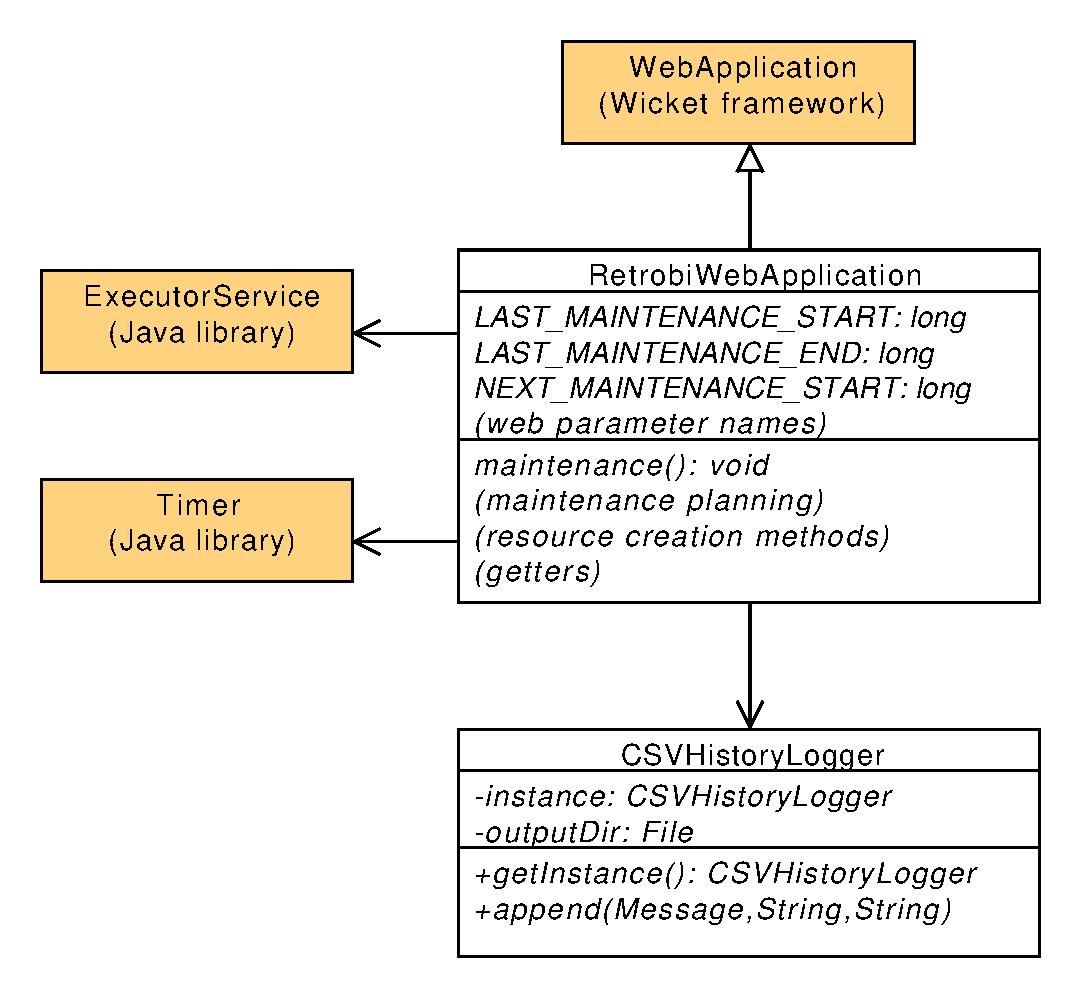
\includegraphics[width=.7\textwidth]{uml_application.pdf}
\caption{webová aplikace (UML)}
\end{figure}

\subsubsection{Stránka, komponenta, model}

Základním objektem frameworku {\em Wicket} je {\em stránka}. Na stánce jsou umístěny komponenty. Komponenty lze seskupovat do větších celků pomocí tzv. {\em kontejnerů} -- speciálních komponent, které mohou obsahovat jiné komponenty. Kontejnerem je například již zmíněná stránka, formulář, panel a další. Vzhled stránek a rozmístění komponent je definován pomocí lehce modifikovaného jazyka XHTML, který zde budeme označovat jako {\em Wicket HTML}. Ten navíc obsahuje tagy pro umisťování komponent.

Při požadavku na danou stránku vezme framework správnou šablonu XHTML, zpracuje ji a postupně ke speciálním tagům přiřadí skutečné instance komponent. 

\begin{verbatim}
Katalog: <h3 wicket:id="nadpis"></h3>
<form wicket:id="formular">...</form>
\end{verbatim}

\begin{verbatim}
add(new Label("nadpis", catalog.getName()));
add(new Form("formular"));
\end{verbatim}

Základními komponentami jsou třídy {\bf Label} (jednoduchý text), {\bf Panel} (panel obsahující samostatnou skupinu spolu souvisejících komponent), {\bf Form} (formulář s ovládacími prvky), {\bf Link} (hypertextový odkaz), {\bf ListView} (panel s opakováním). 

\subsubsection{Hierarchie stránek}

\begin{figure}
\label{fig:pages}
\centering
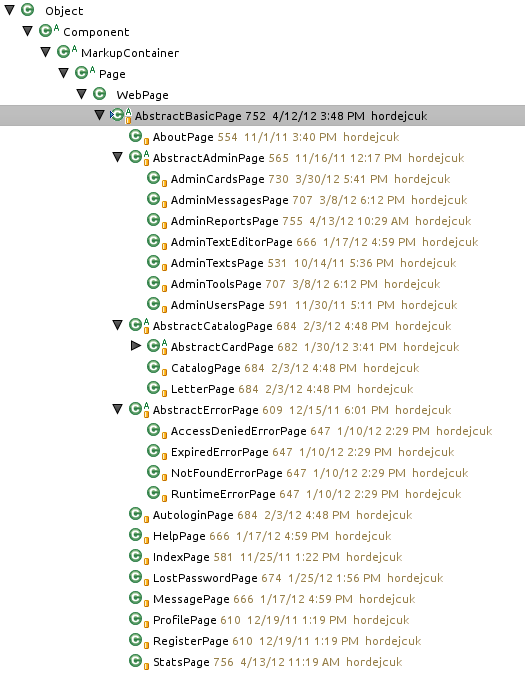
\includegraphics[width=.5\textwidth]{pages.png}
\caption{hierarchie stránek}
\end{figure}

\begin{figure}
\label{fig:uml_cardpage}
\centering
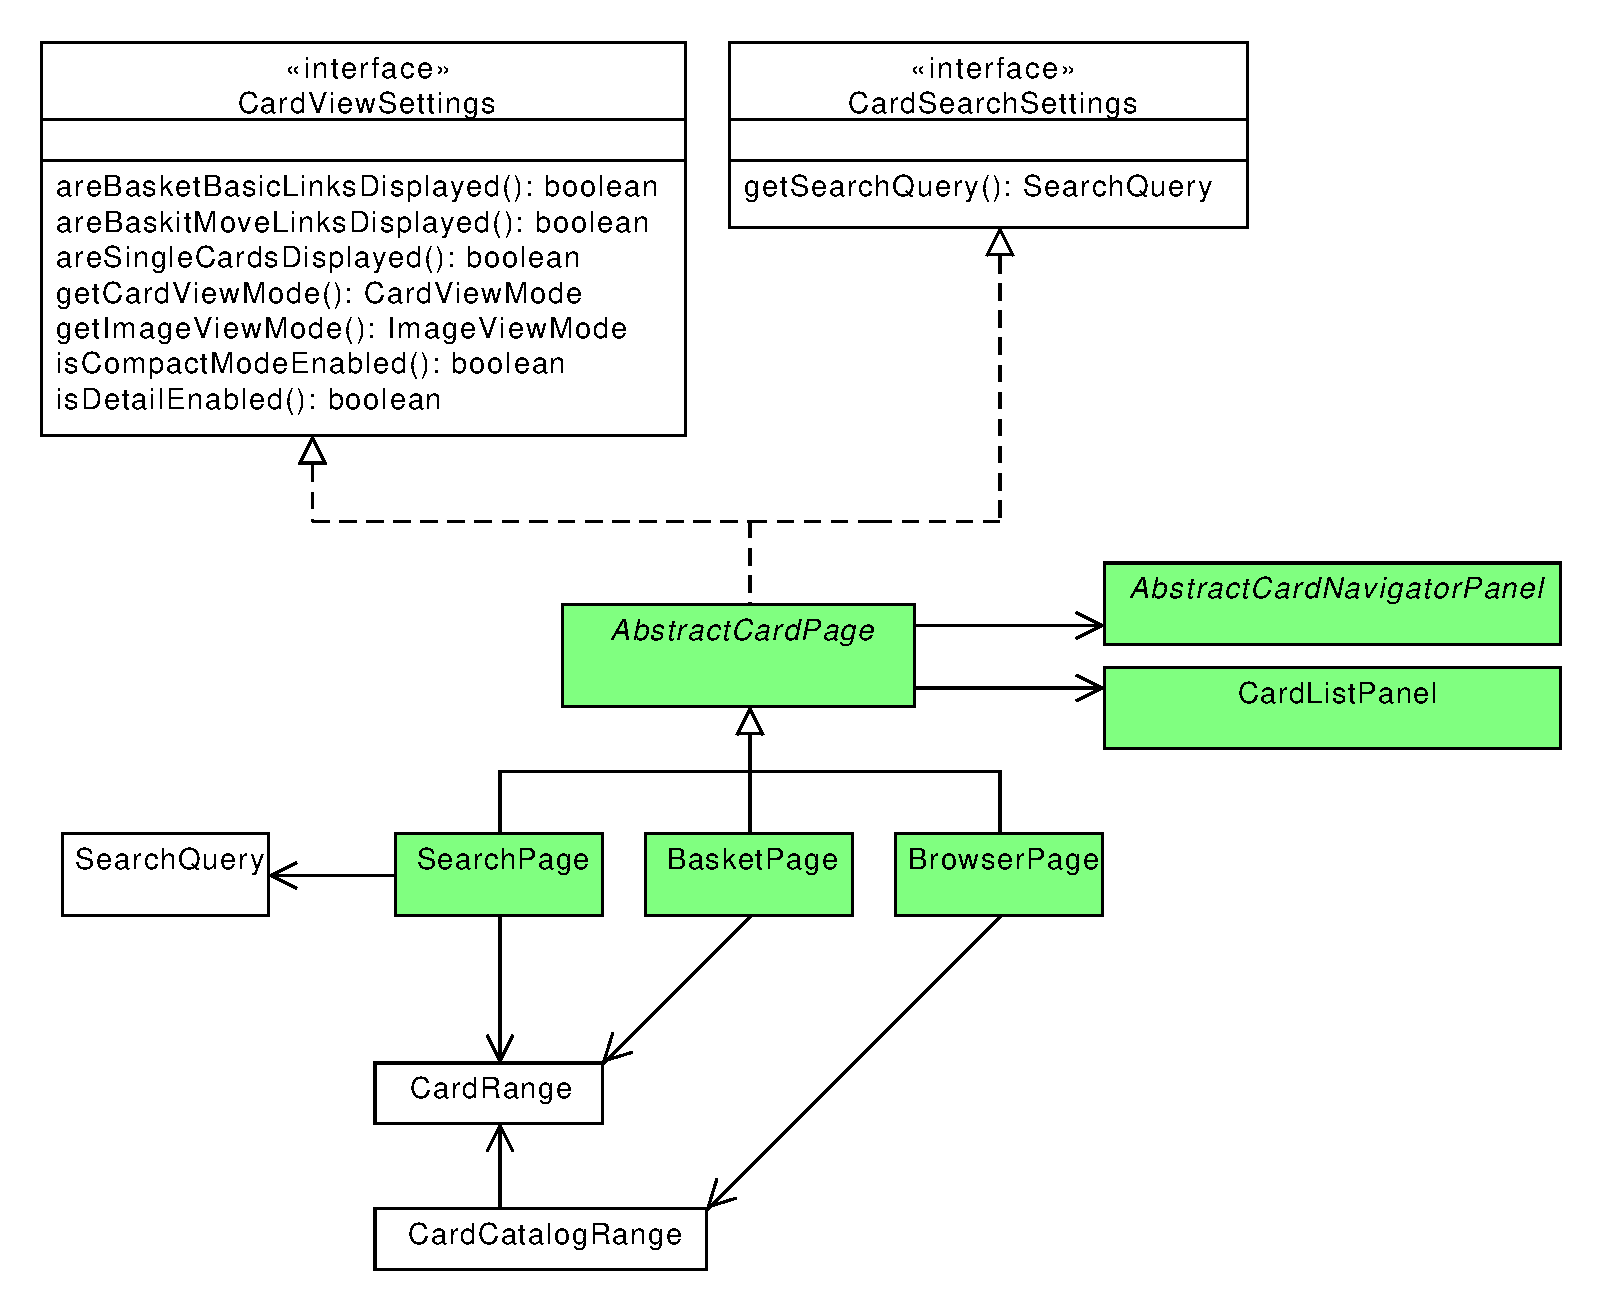
\includegraphics[width=\textwidth]{uml_cardpage.pdf}
\caption{podmnožina tříd vztažených k hlavním stránkám s lístky (zeleně jsou vyznačeny komponenty, tedy vizuální prvky)}
\end{figure}

\subsubsection{Uživatelská relace (Session)} 

\begin{figure}
\label{fig:uml_session}
\centering
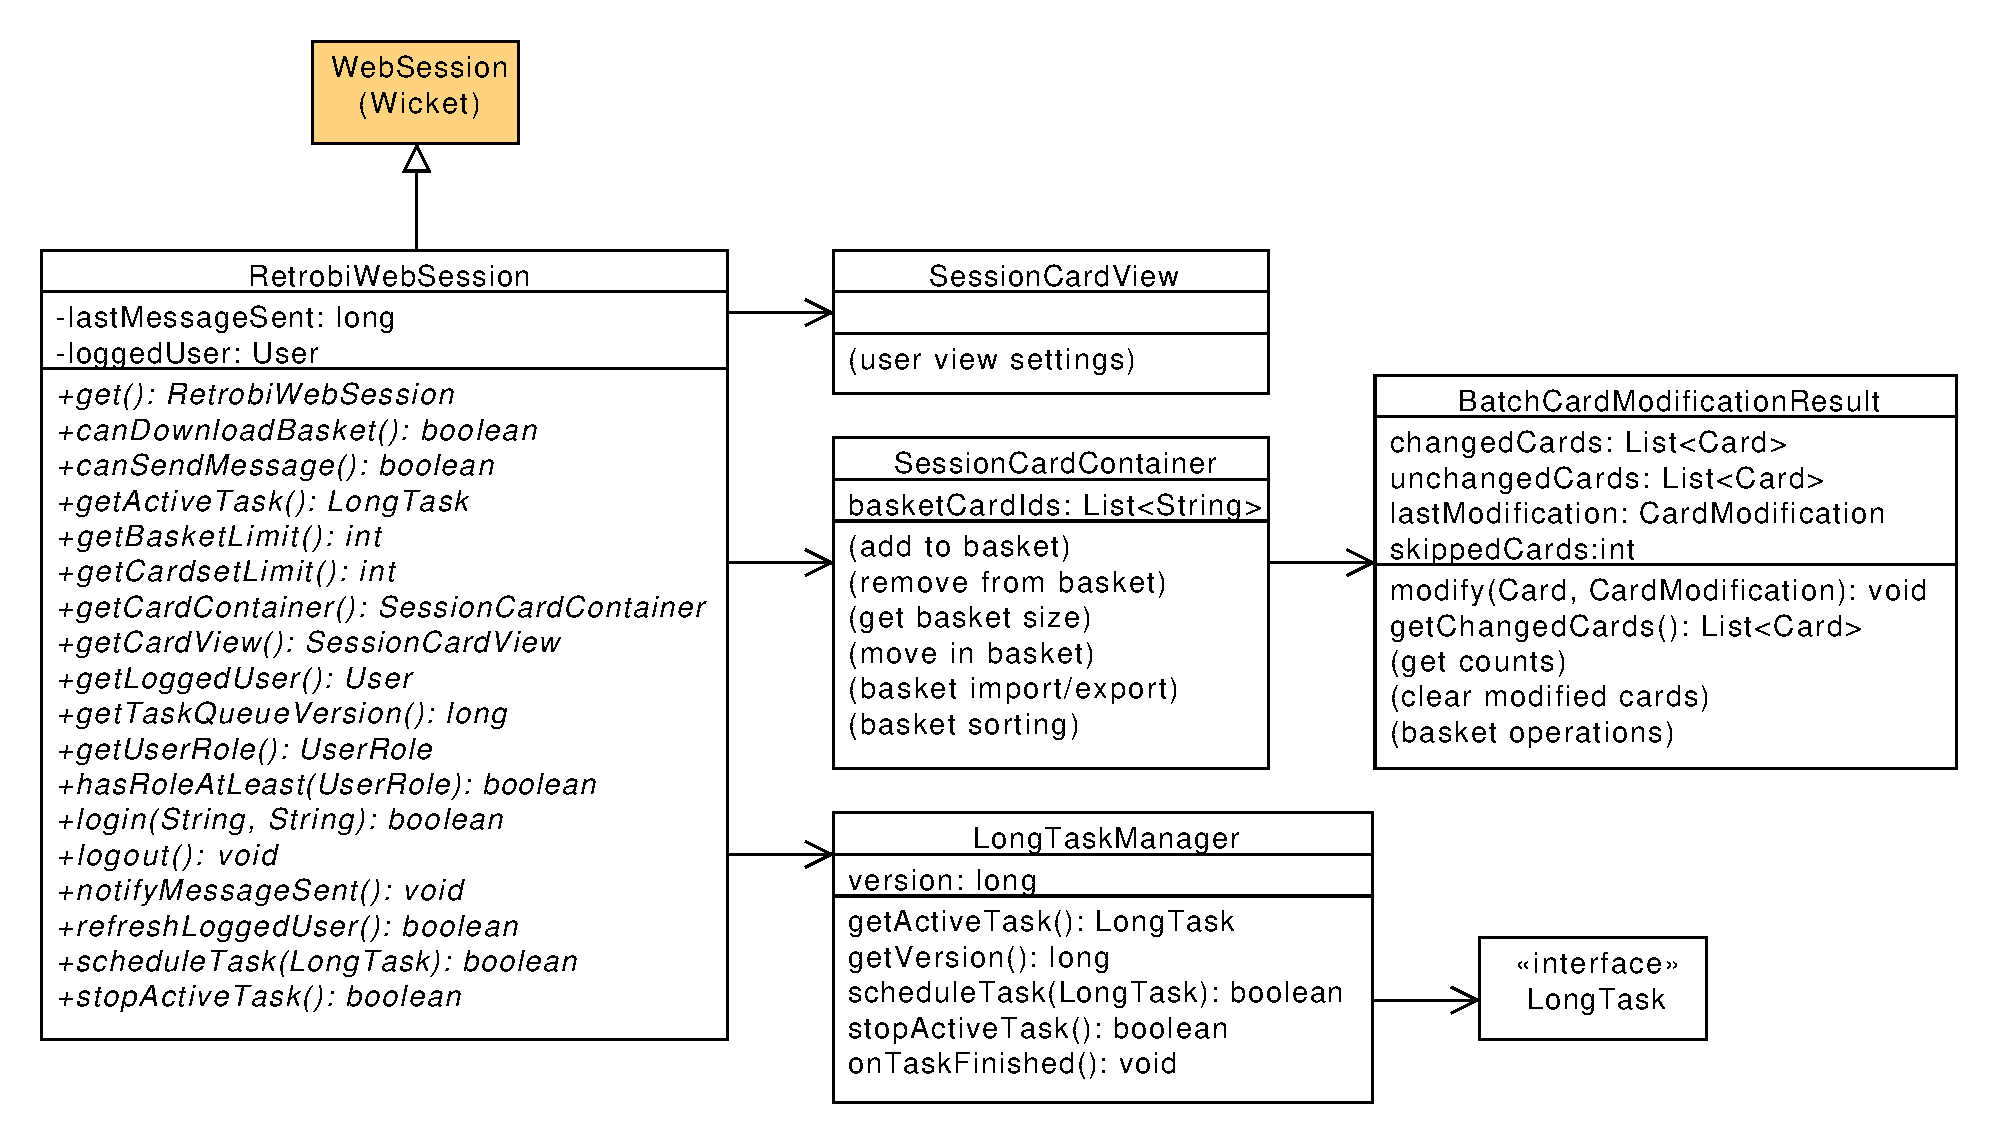
\includegraphics[width=\textwidth]{uml_session.pdf}
\caption{uživatelská relace (UML)}
\end{figure}

Ke každému návštěvníkovi je přiřazena tzv. {\em relace}, což je zjednodušeně řečeno jeho osobní paměťový prostor na serveru. Tato relace je vytvořena, pokud se návštěvník na server připojuje poprvé nebo po dlouhé době.

Každá nová návštěva uživatele vyústí ve vytvoření tzv. {\em relace} (session). Tato relace je následně svázána s konkrétním návštěvníkem (pomocí Cookies) a uchovává se, dokud nevyprší (session timeout, výchozí nastavení je 3 hodiny) nebo není webovým serverem zrušena. 

Klíčovou funkcí relace je uchovávání přihlášení daného uživatele a jeho schránky. Relace dále podporuje dlouhé operace.

\subsubsection{Model katalogu}

Model katalogu je společný pro všechny uživatelské relace, aby se nemusel načítat pokaždé. Model katalogu je jakási cache, obsahující seznam katalogů, skupin, písmen a jejich vzájemné přiřazení. Načtení těchto informací trvá zhruba 5 minut. Model katalogu se proto aktualizuje jen na vyžádání (viz záložka Nástroje ve správě) nebo automaticky při každé denní údržbě.

Abeceda, řazení a ekvivalence písmen je ovlivnitelná jedinou položkou v nastavení, a to pravidly pro řazení písmen. Tato pravidla specifikují, která písmena jsou si \uv{rovna} a jaké je jejich vzájemné pořadí.

Při obnovování katalogu jsou načteny všechny skupiny, seřazeny dle jejich vlastnosti \uv{skupina pro řazení} a dále přiřazeny k jednotlivým písmenům. Vlastnost \uv{skupina pro řazení} je vytvořena při importu lístků do katalogu pomocí nástroje importer a automaticky převádí název skupiny na velká písmena a odstraňuje nepotřebné předložky v příjmení (van, von, aus, de a další).

\subsubsection{Dlouhé úlohy} 

\begin{figure}
\label{fig:uml_task}
\centering
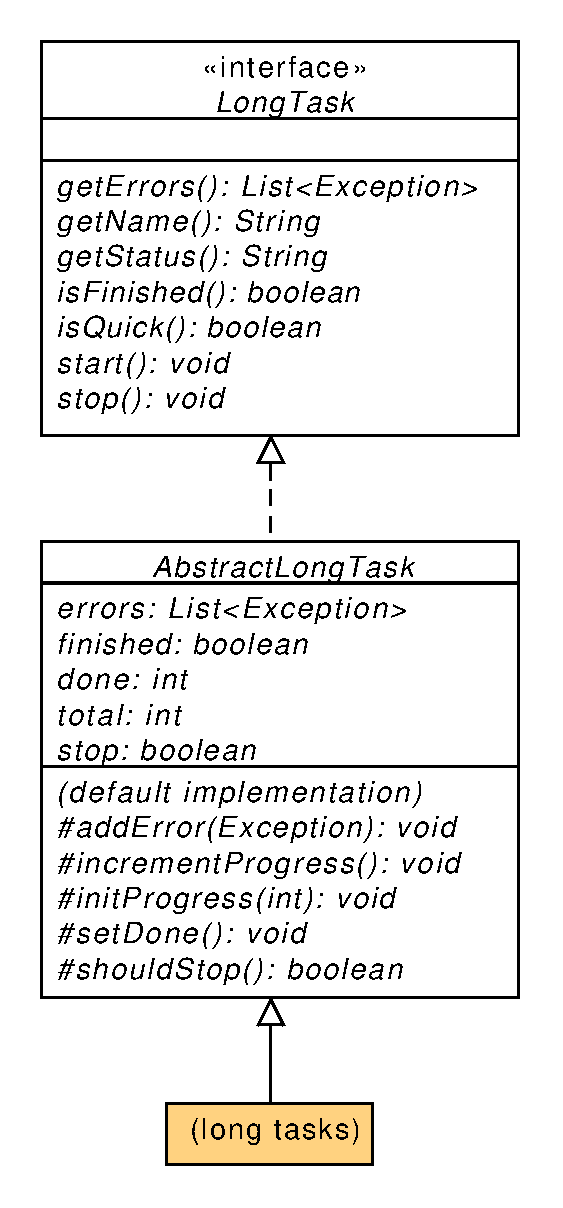
\includegraphics[width=.3\textwidth]{uml_task.pdf}
\caption{dlouhé úlohy (UML)}
\end{figure}

V systému Retrobi existuje několik operací, které obvykle trvají příliš dlouho, než aby byly vykonány během jednoho HTTP požadavku. Pro podobné úlohy byl vytvořen speciální systém, který tyto úlohy řadí do fronty a asynchronně spouští. Webová aplikace obsahuje komponentu, na které je zobrazen stav aktuální úlohy a velikost fronty. Odtud je možné sledovat průběh úlohy, případně ji zastavit. Komponenta se překresluje v pravidelném intervalu pomocí technologie AJAX. Celá stránka se automaticky obnoví po dokončení každé dlouhé úlohy. Chyby vzniklé při provádění úlohy jsou zobrazeny jako klasické informační zprávy do hlavního okna. 

Všechny dlouhé úlohy (tasks) v systému Retrobi implementují rozhraní {\bf LongTask}, které specifikuje metody pro zjišťování stavu úlohy (název, dokončeno, status, chyby), dále pro její zahájení a ukončení. Výchozí implementace některých těchto metod je umístěna ve společném předkovi třídy {\bf AbstractLongTask}, od kterého všechny dlouhé úlohy dědí. Většina dlouhých úloh je spjata s hromadnou editací lístků, která byla popsána výše. Webová aplikace systému Retrobi obsahuje následující dlouhé úlohy:

\begin{description}
\item[AddLetterToBasketTask:]{přidá písmeno do schránky;}
\item[AddSearchToBasketTask:]{přidá výsledek vyhledávání do schránky;}
\item[BatchModificationTask:]{provede hromadnou operaci (obsahuje instanci třídy implementující rozhraní {\bf CardModification} (viz výše), která provede vlastní úpravu každého vybraného lístku);}
\item[DeleteBatchTask:]{smaže zadanou skupinu;}
\item[MultipleCardMoveTask:]{hromadně přesune vybrané lístky na určenou pozici v katalogu;}
\item[RemoveLetterFromBasketTask:]{vyjme písmeno ze schránky;}
\item[RemoveSearchFromBasketTask:]{vyjme výsledek vyhledávání ze schránky;}
\item[SaveBatchModificationTask:]{uloží lístky úspěšně změněné hromadnou operací do databáze;}
\item[SortBasketTask:]{seřadí schránku jako katalog.}
\end{description}

Dlouhé úlohy obsahují i speciální metodu {\bf isQuick()}, která zjišťuje, zda je daná dlouhá úloha nakonec \uv{rychlá} a bylo by možné ji stihnout během jednoho HTTP požadavku. Přesný způsob zjišťování tohoto příznaku je pro každou úlohu jiný. Některé úlohy mohou například považovat za \uv{rychlé} takové instance úloh, které pracují s méně než sto lístky. Tento příznak je využitý v uživatelském rozhraní -- pokud uživatel požádá o spuštění dlouhé úlohy a tato úloha je \uv{rychlá}, není přidána do fronty, ale okamžitě vykonána. To šetří uživatelův čas a ve většina případů zvyšuje předvídatelnost uživatelského rozhraní.

\subsubsection{Automatická údržba}

Při spuštění a každý den v zadanou hodinu (viz konfigurace systému) se spouští tzv. {\em denní údržba}. Během této údržby se vykonají všechny náročnější operace, které z dlouhodobého hlediska vylepšují výkon systému a aktualizují všechna neaktuální data. Během údržby se provedou následující operace: 

\begin{itemize}
\item{Aktualizace položkového rozpisu a definice indexů.}
\item{PING na databázové pohledy (zajistí důslednou aktualizaci všech pohledů).}
\item{Aktualizace model katalogu (katalogy, skupiny a informace o nich).}
\item{Vyčištění indexu od smazaných dokumentů.}
\item{PING a optimalizace všech vyhledávacích indexů (zajistí důslednou aktualizaci všech vyhledávacích indexů).}
\end{itemize}
